%% LLT: Turn off some annoying warnings...
\RequirePackage{silence}
\WarningFilter{titlesec}{Non standard sectioning command}
\WarningFilter{scrreprt}{Usage of package}
\WarningFilter{scrreprt}{Activating an ugly workaround}

% *********************************************************
% CHOOSE THEME (ucph, sund, science, hum, samf, jura, teo)
% *********************************************************
\newcommand{\thesisTheme}{ucph} % to colortheme and titlepage image


% *********************************************************
% DOCUMENT CLASS
% *********************************************************
\documentclass[%
	paper=A4,					% paper size
	12pt,						% font size
	twoside=true,				% two-sided printing
	openright,					% doublepage cleaning ends up right side
	parskip=full,				% spacing value / method for paragraphs
	chapterprefix=true,			% prefix for chapter marks
	headings=normal,			% size of headings
	bibliography=totoc,			% include bib in toc
	listof=totoc,				% include listof entries in toc
	titlepage=on,				% own page for each title page
	captions=tableabove,		% display table captions above the float env
	draft=false,				% value for draft version
	abstract=on,
	% abstract title on/off
]{scrreprt}
\usepackage[utf8]{inputenc}
\usepackage[english]{babel}     % adjust the language
\usepackage{amsmath}
\usepackage[autostyle]{csquotes}
\usepackage{amssymb}
\usepackage{caption}
\usepackage[ruled,vlined,linesnumbered]{algorithm2e}
\usepackage{scalerel,stackengine}
\usepackage{csvsimple}
\usepackage{array}
\usepackage{graphics}
\usepackage{mathtools}
\stackMath
\newcommand\reallywidehat[1]{%
\savestack{\tmpbox}{\stretchto{%
  \scaleto{%
    \scalerel*[\widthof{\ensuremath{#1}}]{\kern-.6pt\bigwedge\kern-.6pt}%
    {\rule[-\textheight/2]{1ex}{\textheight}}%WIDTH-LIMITED BIG WEDGE
  }{\textheight}% 
}{0.5ex}}%
\stackon[1pt]{#1}{\tmpbox}%
}
% **************************************************
% COMMANDS FOR REUSE
% **************************************************

% Thesis
\newcommand{\thesisTitle}{Learning network design solution
strategies using reinforcement learning}
\newcommand{\thesisSubtitle}{an
application to multicommodity capacitated fixed-charge network design problem}
\newcommand{\thesisName}{Sangmin Lee}
\newcommand{\thesisSubject}{MSc in Statistics}
\newcommand{\thesisDate}{August 2020}
\newcommand{\thesisVersion}{First Version}

% Supervisors & Collaborators
\newcommand{\thesisExternalSupervisor}{Klaus K{\"a}hler Holst}
\newcommand{\thesisInternalSupervisor}{Trine Krogh Boomsma}
\newcommand{\thesisCollab}{A. P. M{\o}ller - M{\ae}rsk A/S}

% University of Copenhagen
\newcommand{\thesisUniversity}{\protect{University of Copenhagen}}
\newcommand{\thesisFaculty}{Faculty of Sciences}
\newcommand{\thesisInstitute}{Masters Degree in Statistics}
\newcommand{\thesisCity}{Frederiksberg}
\newcommand{\thesisAddress}{B{\"u}lowsvej 17}
\newcommand{\thesisPostal}{1870}

% External institution: University of Sussex
\newcommand{\thesisUniSus}{\protect{University of Sussex}}
\newcommand{\thesisUniSusDep}{Department of Life Sciences}


% *********************************************************
% PACKAGES
% *********************************************************

\usepackage[					% UCPH thesis style
    figuresep=colon,        
    sansserif=false,        
    hangfigurecaption=false,
    hangsection=true,       
    hangsubsection=true,    
    colorize=full,          
    colortheme={\thesisTheme},  % ucph, sund, science, hum, etc.?
    bibsys=biber,
    bibfile=references,       % defines your .bib file
    bibstyle=authoryear,        % refer to https://bit.ly/2YsvIJz
]{ucphthesis}
\hypersetup{					% setup the hyperref-package options
	pdftitle={\thesisTitle},	% 	- title (PDF meta)
	pdfsubject={\thesisSubject},% 	- subject (PDF meta)
	pdfauthor={\thesisName},	% 	- author (PDF meta)
	plainpages=false,			% 	-
	colorlinks=false,			% 	- colorize links
	pdfborder={0 0 0},			% 	-
	breaklinks=true,			% 	- allow line break inside links
	bookmarksnumbered=true,		%
	bookmarksopen=true			%
    }

% *********************************************************
% Cover page content
% *********************************************************
\subject{\vspace{4.5cm} \thesisSubject}
\title{\thesisTitle}
\subtitle{\thesisSubtitle}
\author{\thesisName \\
        \small{Supervised by {\thesisExternalSupervisor} and {\thesisInternalSupervisor}}
    }
\date{\thesisDate}


% ********************************************************* 
% THESIS CONTENT
% *********************************************************
\begin{document}

% -------------------------- 
% Front matter
% --------------------------
\pagenumbering{roman}
\pagestyle{empty}				            % no header or footers
%\AddToShipoutPicture*{\TitleBackground}     % adding background picture
%\maketitle                                  % making the title
%% Cover back page
\AddToShipoutPicture*{\TitleWatermark}% adding watermark
\hfill
\vfill
{
	\small
	\textbf{\thesisName} \\
	\textit{\thesisTitle} \\
	\thesisSubject, \thesisDate \\
	Supervisors: \thesisExternalSupervisor\ and \thesisInternalSupervisor \\
	External Partners: \thesisCollab \\[1.5em]
	\textbf{\thesisUniversity} \\
	\textit{\thesisFaculty} \\
	\thesisInstitute \\
	\thesisAddress \\
	\thesisPostal\ \thesisCity
}

    \clearpage

\pagestyle{plain}
%\vspace*{4cm}
\textit{"I want."} \\
\newline
\rightline{August Krogh, 1929 \nocite{Krogh1929}} \\
\vspace{2cm}
\newline
\textit{"It is certain"} \\
\newline
\rightline{C, 1872 \nocite{Darwin1872TheSex}}
\vspace{3.8cm}


        % INCLUDE Quotes
%\pdfbookmark[0]{Preface}{Preface}
\chapter*{Preface}
\label{chap:preface}
In the preface, you inform the reader about your experiences during the writing of your dissertation. You can also use the preface to help the reader get started and to thank people who have helped you with your dissertation.
Your personal background (in brief)
Your personal experiences or the circumstances that motivated you to write your dissertation (in brief)
The target group for which your dissertation was written
The division of labor (when the dissertation has been written by more than one person)
Acknowledgements to individuals and institutions who have helped you in the writing and checking of the dissertation
The preface ends with you name,  place name, and date at the time of writing.
%\vspace*{5cm}       % INCLUDE Preface
%\pdfbookmark[0]{Acknowledgements}{Acknowledgements}
\chapter*{Acknowledgements}
\label{chap:acknowl}
 % INCLUDE Acknowledgements
%\pdfbookmark[0]{Abstract}{Abstract}
\chapter*{Abstract}
\label{chap:abstract}
An abstract is a short summary that appears at the start of a longer work, such as a dissertation, research paper or journal article. To write an abstract, you should:
Introduce your topic and objectives
Briefly describe your methods
Summarize your key results or arguments
State your conclusion
The abstract allows potential readers to quickly see what your paper is about and decide if it’s worth reading. It is usually around 150–300 words, but there’s often a strict word limit, so make sure to check the requirements.      % INCLUDE Abstract
    \clearpage


\setcounter{tocdepth}{2}		% define depth of toc
\tableofcontents				% display table of contents
    \clearpage


% -------------------------- 
% Main matter
% --------------------------
\pagenumbering{arabic}			% arabic page numbering
\setcounter{page}{1}			% set page counter
\pagestyle{maincontentstyle} 	% fancy header and footer

%\chapter{Rationale}
\label{chap:rationale}

Locomotion is thought to be a tightly controlled behaviour, ensuring good sensory performance, especially visual, and reducing energy expenditure \autocites{Benichou2011IntermittentStrategies, Kramer2001}. Whether this is the case in the wood ant \textit{Formica rufa} remains unknown, despite many aspects of ant locomotion having been well studied \autocites{Lipp2005, Wahl2015}. The wood ant is an eusocial insect capable of using vision for navigation \autocite{Harris2007} and associative learning \autocite{Fernandes2017a}. Furthermore, other ant species have been found able to use optic flow for path integration (\textit{Cataglyphis}, \citealt{Ronacher1995, Pfeffer2016}). It could thus be speculated that vision actively controls general walking features such as speed, duration and pausing in the wood ant, \textit{Formica rufa} (like bees control speed, \cite{Schone1996, Linander2015}). We ask the following question: Does control of walking speed and pausing depend on the presence and speed of optic flow?

A promising approach for performing behavioural experiments in a laboratory setting is the use of virtual reality. Insects have recently been shown to exhibit naturalistic behaviour in closed-loop within a virtual environment \autocites{Takalo2012, Buatois2017, Seelig2010}. Such setups allow data sampling at precise temporal and spatial resolution whilst animals walk unrestricted for long periods of time. They further enable the recording of brain activity directly, either by electrophysiological recordings or calcium imaging \autocite{Seelig2010}. However, despite continued efforts from multiple laboratories it has not yet been possible to make a setup in which ants will readily behave within closed-loop. Nevertheless, we set out to develop a virtual reality paradigm for wood ants (\textit{Formica rufa}). We propose a paradigm based on a modified closed-loop version of the trackball setup by \citeauthor{Dahmen2017} (\citeyear{Dahmen2017}) combined with the virtual reality software developed by \citeauthor{Aronov2014b} (\citeyear{Aronov2014b}).     INCLUDE Rationale
\part{Preliminaries}
\chapter{Introduction}
\label{chap:intro}
\vspace{1cm}

A \textit{combinatorial optimization} (CO) problem is a problem of either minimizing or maximizing a real-valued \textit{objective function} on a finite set of feasible solutions $\mathcal{S}$, which is comprised of all subsets of some finite \textit{ground set} $E$ (\citeauthor{lee_2004} \cite{lee_2004}). The CO problem can often be formulated as an optimization program with constraints. A problem is called a linear programming (LP) if both objective function and constrains are linear, and a mixed-integer linear programming (MILP) if an integrality constraint is additionally imposed on some of decision variables in the objective function. In many practical cases, CO is used to formulate problems that arise in industry, such as transportation, manufacturing, telecommunication, energy, and finance (\citeauthor{bengio2018machine} \cite{bengio2018machine}; \citeauthor{lee_2004} \cite{lee_2004}). Many of such problems, however, are NP-hard, which means that finding a solution to them is at least as hard as solving NP-complete problems --- the most difficult problems in NP where solutions can be verified in polynomial time (\citeauthor{paarsch2016gentle} \cite{paarsch2016gentle}). Due to their worst-case complexity, there is no known algorithms that produce the optimal solution to the NP-hard problems in polynomial time unless $P = NP$, and thus great attention has been paid to finding efficient methods to tackle NP-hard problems (\citeauthor{barrett2019exploratory} \cite{barrett2019exploratory}). % approximately 180 words (100-200 words)

To handle NP-hard CO problems, there have been introduced three classic approaches: exact algorithms, approximation algorithms and heuristics. Exact algorithms, which are based on enumeration or branch-and-bound, find the optimal solution by searching the whole solution space; however, this method becomes intractable for a large problem. A polynomial-time approximation algorithm, on the other hand, produces a solution that is close to the optimal solution in polynomial time for all instances of the problem, but there still remain a number of problems that have no polynomial-time approximation algorithm (\citeauthor{williamson2011design} \cite{williamson2011design}). In practice,  heuristics are often used for solving a large problem, as they may perform more quickly than the other two classic approaches. This method, however, provides no theoretical guarantees, meaning that it may converge to a local optimal solution (\citeauthor{barrett2019exploratory} \cite{barrett2019exploratory}; \citeauthor{williamson2011design} \cite{williamson2011design}).

In addition to these three traditional methods, recent years have witnessed the increase of using a machine learning (ML) method to handle NP-hard CO problems. \citeauthor{bengio2018machine} \cite{bengio2018machine} introduced two motivations for developing CO algorithms based on the ML technique. Given a CO problem in a high-dimensional space, ML can enhance an expert intuition on optimization algorithms by substituting a fast approximation, such as deep learning architectures, for heavy computations. Moreover, ML may bring a new insight into the best performing algorithm by exploring the whole decision space. A recent work by \citeauthor{silver2017mastering} \cite{silver2017mastering} has viewed these two motivations through a successful experiment on their computer program, AlphaGo, which defeats a world champion Go player in 2016. To tackle heavy computations of evaluating board positions and moves, deep neural networks and Monte Carlo tree search are employed in AlphaGo, and its policy network is trained on human expert games (\citeauthor{silver2016mastering} \cite{silver2016mastering}).

There have been developed numerous learning-based methods for solving NP-hard CO problems on graphs.

4th paragraph - Brief description of our methods and MCFND.

5th paragraph - Brief description of our experiments and results.

6th paragraph - "Overall our paper makes the following contributions"

7th paragraph - "The rest of the paper is structured as follows. In chapter ~"

\chapter{Related Work}
\label{chap:related_work}
\vspace{1cm}

A reinforcement learning approach to solving NP-hard CO problem was pioneered in the nineties by \citeauthor{zhang1995reinforcement} \cite{zhang1995reinforcement}, who demonstrate how the temporal difference algorithm TD($\lambda$) can be applied to job shop scheduling problems, in particular a NASA space shuttle payload processing task. They compare the performance of TD method (\citeauthor{sutton1988learning} \cite{sutton1988learning}) to that of the Zweben's iterative repair (IR) method (\citeauthor{zweben1993scheduling} \cite{zweben1993scheduling}), which was then the best known algorithm for such problem, and show that TD scheduling produces better solution with less running time.

Recently, \citeauthor{bello2016neural} \cite{bello2016neural} combined neural networks with a reinforcement learning to solve CO problems on graphs, particularly the traveling salesman problem (TSP) with up to 100 nodes. Their idea is to train neural networks with the reinforcement learning, rather than a supervised learning. Based on REINFORCE algorithm, which is a policy-gradient learning method proposed by \citeauthor{williams1992simple} \cite{williams1992simple}, \citeauthor{bello2016neural} presented two approaches -- RL pretraining and active search -- and used pointer networks (\citeauthor{vinyals2015pointer} \cite{vinyals2015pointer}) as their policy model. Their experiments on TSP showed that the reinforcement learning outperforms the supervised learning in training pointer networks. Moreover, their RL pretraining methods produce better results compared to OR-tool's local search.

The framework presented in \citeauthor{bello2016neural} \cite{bello2016neural}, however, did not effectively reflect the graph structure of CO problems defined on graphs, such as connectivity and the problem's constraints. \citeauthor{khalil2017learning} \cite{khalil2017learning} handled such challenge with a graph embedding network. They proposed

\citeauthor{kool2018attention} \cite{kool2018attention}

\citeauthor{li2018combinatorial} \cite{li2018combinatorial}

\citeauthor{ma2019combinatorial}\cite{ma2019combinatorial}

\citeauthor{barrett2019exploratory} \cite{barrett2019exploratory}

\citeauthor{li2019learning} \cite{li2019learning}

\citeauthor{nazari2018reinforcement} \cite{nazari2018reinforcement}


$\#\#$ Multi-RL

\part{Materials and Methods}
\chapter{Network Design}
\label{chap:Network Design}
\vspace{1cm}

Network design problems have important applications in transportation planning, since it can represent the most essential features of transportation systems: ``strategic, tactical, and operational decision-making situations'' (\citeauthor{magnanti1984} \cite{magnanti1984}, p.1). This chapter is devoted to a network design problem that we attempt to solve --- an unsplittable multicommodity capacitated fixed-charge network design (UMCFND) problem. In \autoref{sec: UMCFND formulation} we fomulate the UMCFND problem, and we briefly discuss how it can be applied to the  transportation planning in \autoref{sec:applictions of UMCFND}.

The UMCFND problem is a variant of a multicommodity capacitated fixed-charge network design (MCFND) problem (\citeauthor{gendron1994} \cite{gendron1994}), where the flow of each commodity is not split. That is, in the UMCFND problems, each commodity must be transported along a single path only. The objective of UMCFND problems is to optimize the total expenses consisting of the cost of shipping goods and the construction cost of edges while each commodity is delivered to its destination depot from its orgin depot along a single capacitated path. Thus, it can be viewed as an extension of the classic multicommodity flow problems (\citeauthor{ahujia1993network} \cite{ahujia1993network}) by forbidding the flow to split and introducing binary design variables which decide whether to include each edge in a network design model.

When the construction cost of an edge is not considered the problem becomes an origin-destination integer multicommodity flow (ODIMCF) problem (\citeauthor{barnhart2000using} \cite{barnhart2000using}). In this paper, we are given a directed graph $G = (V, E)$, where $V$ and $E$ is the set of nodes and edges, respectively.

\section{UMCFND Problem Formulation}
\label{sec: UMCFND formulation}
In this section, we describe the formulation of the UMCFND problem using the following notations.
\subsubsection*{Notations}
\begin{table}[!htbp]
\begin{tabular}{ccl}
    $V$ & & set of nodes in the network \\[0.5em]
    $E$ & & set of edges \\[0.5em]
    $\mathcal{K}$ & & set of commodities to be conveyed\\[0.5em]
    $O(k)$ & & origin node for each commodity $k$\\[0.5em]
    $D(k)$ & & destination node for each commodity $k$ \\[0.5em]
    $d^k$ & & nonnegative quantity of each commodity $k$\\[0.5em]
    $c_{ij}^k$ & & nonnegative unit flow cost of commodity $k$ on edge ($i$, $j$)\\[0.5em]
    $f_{ij}$ & & nonnegative fixed design cost for edge ($i$, $j$)\\[0.5em]
    $u_{ij}$ & & positive capacity on edge ($i$, $j$)\\[0.5em]
\end{tabular}
\end{table}
\begin{align*}
    x_{ij}^k &=
    \begin{cases}
    \ 1 & \text{if the entire quantity } d^k \text{ of commodity } k \text{ is assigned to edge }(i,j), \\
    \ 0 & \text{otherwise}.
    \end{cases}
    \\
    y_{ij} &=
    \begin{cases}
    \ 1 & \text{if edge } (i, j) \text{ is included in the network design}, \\
    \ 0 & \text{otherwise}.
    \end{cases}
\end{align*}

\vfill

\subsubsection*{Formulation of UMCFND}
The UMCFND problem can be formulated as an integer linear program:
\begin{itemize}
    \item\textit{Objective function}
    \label{eq:obf}
        \begin{align}
            \text{minimize}\qquad &\sum_{k\in \mathcal{K}}\sum_{(i,j)\in E} c_{ij}^k d^k x_{ij}^k + \sum_{(i,j)\in E} f_{ij}y_{ij}
        \end{align}
        
    \item\textit{Flow conservation constraints}
        \begin{align}
        \label{eq: Conservation constraints}
            \sum_{(i,j)\in E}x_{ij}^k - \sum_{(j,i)\in E}x_{ji}^k = 
            \begin{cases}
            \ 1 & \text{if } i = O(k),\\
            \ -1 & \text{if } i = D(k),\\
            \ 0 & \text{if } i \neq O(k), i \neq D(k),\\
            \end{cases} \ \  \forall i \in V, \forall k \in \mathcal{K}
        \end{align}
        
    \item\textit{Capacity constraints}
        \begin{align}
        \label{eq:Capacity constraints}
            \sum_{k\in \mathcal{K}} d^kx_{ij}^k \leq u_{ij}y_{ij}, \qquad \forall (i, j) \in E
        \end{align}

    \item\textit{Bounding constratints on design variables}
        \begin{align}
            &x_{ij}^k \leq 1, \qquad  \forall (i, j) \in E, \quad\forall k \in \mathcal{K},\label{eq:Bounding on design var1}\\
            &y_{ij} \leq 1, \qquad  \forall (i, j) \in E
        \end{align}
        
    \item\textit{Nonnegativity constraints on design variables}
        \begin{align}
        \label{eq:Nonnegativity on design var}
            &x_{ij}^k \geq 0, \qquad  \forall (i, j) \in E, \quad\forall k \in \mathcal{K},\\
            &y_{ij} \geq 0, \qquad  \forall (i, j) \in E
        \end{align}
    
    \item\textit{Integrality constraints on design variables}
        \begin{align}
            &x_{ij}^k \ \text{ integer},\qquad  \forall (i, j) \in E, \quad\forall k \in \mathcal{K},\\
            &y_{ij} \ \text{ integer}, \qquad  \forall (i, j) \in E \label{eq:Integrality on design var2}
        \end{align}
\end{itemize}

The objective function, \eqref{eq:obf}, minimizes the sum of transportation cost of all commodities shipped to their destinations from their origins plus fixed costs of the constructed edges. The flow conservation constraints, \eqref{eq: Conservation constraints}, ensure that the flow of each commodity is routed using a single path from its origin node to its destination node. The capacity constraints, \eqref{eq:Capacity constraints}, limit the total flow on an open edge to its capacity, but also it states that the amount of flow on the closed edge must be zero until the fixed cost is paid. Constraints \eqref{eq:Bounding on design var1} -- \eqref{eq:Integrality on design var2} specify the nature of design variables.

\section{UMCFND in Transportation Planning}
\label{sec:applictions of UMCFND}

\citeauthor{gendron2011} \cite{gendron2011} argue that the MCFND model has three crucial properties: the interaction between investment and operating expenses, aspects of the multiple commodities, and the capacity factor. With this regard, variants of the MCFND have been widely applied to the transportation planning. For instance,  \citeauthor{yaghini2012multicommodity} \cite{yaghini2012multicommodity} discuss applications of the MCFND in rail freight transportation planning, and \citeauthor{krile2004application} \cite{krile2004application} deals with applying the minimum cost multicommodity flow problem to finding an optimal plan of container shipping.

A commodity is often conveyed along a single network path for greater operational efficiency and customer satisfaction (\citeauthor{barnhart2000using} \cite{barnhart2000using}). In this case, we can make good use of the UMCFND problem.

As a global logistics service provider, solving the UMCFND problem may contribute to developing our business strategy, since it plays a critical role in coordinating shipments and building shipping routes economically. 
\clearpage
\chapter{Single-Agent Reinforcement Learning}
\label{chap:Reinforcement Learning}
\vspace{1cm}

In this chapter we introduce a reward-driven trial-and-error learning method, which is called \textit{reinforcement learning}, with a single agent in particular, and illustrate how to apply reinforcement learning to CO problems on graphs.

To describe the general idea of reinforcement learning, let us first consider a delivery truck shipping products from city \texttt{A} to city \texttt{B}, displayed as in \autoref{fig:delivery truck}. We assume that there are three different routes (route \texttt{a}, route \texttt{b}, route \texttt{c}) between those two cities, and they have different transportation cost, as in \autoref{fig:delivery truck}. To find the least-cost path, the delivery truck tries every route, records how much it costs the truck, and compare them. Here, the negative of transportation cost can be thought of as a reward. Eventually, the delivery truck learns that the route \texttt{c} produces the largest reward, and thus, it will always use the route \texttt{c} afterwards.
\begin{figure}[hbt!]
    \centering
    \includegraphics[width=0.65\textwidth]{figures/Reinforcement/truck.png}
    \captionsetup{justification=centering}
    \caption{Delivery truck example}
    \label{fig:delivery truck}
\end{figure}

The idea behind reinforcement learning is that its learning mechanism is driven by rewards from the environment a learning agent is interacting with. In order to maximize the reward, the agent learns what is the best decision to make from its experience of receiving a reward from the environment.

In our delivery truck example, the truck takes an action, which is to choose a specific route, and receives a corresponding reward -- the negative of transportation cost. The environment here can be considered as a function of a current city and action that returns a reward and the next city. For instance, if the delivery truck takes an action to select the route \texttt{a} from the city \texttt{A}, then the environment returns the city \texttt{B} and the reward -10. At the end, the delivery truck learns that choosing the route \texttt{c} is the best action to maximize the reward.

Reinforcement learning can be characterized by three noteworthy features. First of all, a learning agent has no instructor who directs which actions to choose, and thus, should try various actions until it discovers the best one that provides the biggest reward. Second, the main objective of reinforcement learning is to maximize the total amount of reward received from the environment, rather than investigate the hidden structure of unlabeled data. Finally, the agent has to \textit{exploit} the past experience to select the best action that offers the greatest reward, but also to \textit{explore} undiscovered actions for better rewards in the long run. To maximize a reward, a learning agent prefers to select actions that have yielded the most rewards from what has already been executed so far. The agent, however, has also to try other actions that have not been chosen in the past, since one of them may produce the biggest reward among all actions.

In our delivery truck example, no one tells which route should be taken, and thus, the truck explores all three routes to discover the least-cost route. Moreover, The delivery truck does not look into the transportation cost mechanism, but merely tries to maximize its reward. To describe the last key feature of reinforcement learning from the delivery truck example, let us assume that the truck has only tried the route \texttt{a} and route \texttt{b} at this moment. If the truck does not go further in its exploration of finding the best route and only exploits its past experience, then it will end up with choosing the route \texttt{a} as the best route, which is not true. Since it is impossible to perform both exploitation and exploration with a single action, the agent should balance them during the learning process to achieve the greatest reward at the end.

The first section of this chapter describes a \textit{Markov Decision Process} (MDP), which is a mathematical framework for designing problems where reinforcement learning methods with a single agent can be applied, and illustrates how a single-pair shortest path problem fit into this framework. In \autoref{sec: Tabular Solution Method}, we introduce a temporal-difference learning method, which is one of reinforcement learning methods for solving finite Markov decision problems. In particular, we look more closely at its off-policy case, which is known as Q-learning (\citeauthor{watkins1989learning} \cite{watkins1989learning}), and solve our single-pair shortest path problem using Q-learning. In \autoref{sec: value function approximation}, we extend the temporal-difference learning method with function approximation so that it can handle problems whose state space is significantly large. In \autoref{}


\section{Markov Decision Processes}
\label{sec: Markov Decision Process}
In this section, we present how to formulate reinforcement learning problems of maximizing cumulative reward with a single agent using the framework of Markov decision processes (MDPs), which comes from the field of optimal control. In reinforcement learning, much attention is given to cases where we approximate an optimal solution that is hard to find, and the exact model of problem is unknown. For more detailed discussion of historical influences of MDPs on reinforcement learning, see Chapter 1 and 3 of \citeauthor{sutton2018reinforcement} \cite{sutton2018reinforcement}.

Moreover, we consider a toy example of single-pair shortest path problem with an undirected graph, presented as in \autoref{fig:toy graph}, where it aims to find a path between origin node to destination node such that the sum of the transportation cost of its consisting edges is minimized.

\begin{figure}[hbt!]
    \centering
    \includegraphics[width=0.95\textwidth]{figures/Reinforcement/figure1.png}
    \caption{\textbf{Example 1}: the shortest path is represented by the bold line. The number next to the edge is its transportation cost.}
    \label{fig:toy graph}
\end{figure}
\clearpage
\subsection{The Agent-Environment Interface}
The one who learns and makes a decision is called the \textit{agent}, and the world where the agent moves around is composed of three elements: set of all states, $\mathcal{S}$, set of all actions available in state $s \in \mathcal{S}$, denoted by $\mathcal{A}(s) \subset \mathcal{A}$, and set of all possible rewards, which is a subset of real number set, $\mathcal{R} \subset \mathbb{R}$.

\begin{figure}[hbt!]
    \centering
    \includegraphics[width=0.7\textwidth]{figures/Reinforcement/interaction.pdf}
    \captionsetup{justification=centering}
    \caption{Agent-environment interaction}
    \label{fig:interaction}
\end{figure}

The system that the agent interacts with is called the \textit{environment}. To describe this more specifically, let us assume that the agent interacts with the environment at each of a sequence of discrete time steps, $t = 0,1,2, \dots$. At each time step $t$, the agent is given at a state $S_t \in \mathcal{S}$, and selects an action $A_t \in \mathcal{A}(S_t) \subset \mathcal{A}$, which is available in a given state $S_t$, and then two pieces of information, $(S_t, A_t)$, are transmitted to the environment. In the next time step, the environment grants the agent a reward $R_{t+1} \in \mathcal{R}$ and a new state, $S_{t+1}$. The process of agent-environment interaction is displayed in \autoref{fig:interaction}. A \textit{trajectory} that arises from such interaction can be illustrated by a sequence as follows:
\begin{align}S_0, A_0, R_1, S_1, A_1, R_2, S_2, A_2, R_3, S_3, \dots\end{align}
If states, actions, and rewards in MDP are discrete random variables with finite support, then it is called a \textit{finite} MDP. Let us now define \textit{state-reward-transition} probability function $p : \mathcal{S}\times\mathcal{R}\times\mathcal{S}\times\mathcal{A}\rightarrow[0,1]$ as follows:
\begin{align}
\label{eq:dynamics function}
p(s',r|s,a) := \text{Pr}\{S_t=s', R_t=r \ | \ S_{t-1} = s, A_{t-1} = a\},
\end{align}
for all $s',s\in \mathcal{S}, r\in\mathcal{R}$, and $a\in\mathcal{A}(s)$. The function $p$ provides a probability density function of $S_t$ and $R_t$, conditioning on the preceding state and action ($S_{t-1}$, $A_{t-1}$). This probability function $p$ defines the environment in reinforcement learning problems with a single agent.

Equation \eqref{eq:dynamics function} implies that the probability of each possible state and reward at a time step $t$ depends only on the value of $S_{t-1}$ and $A_{t-1}$, and thus, it is independent of all the states and actions that had happened before a time step $t-1$. Throughout this paper, we will assume that all the information about agent-environment interactions that occurred in the past must be reflected in the current state, which is then said to have the \textit{Markov property}.

From the four-argument state-reward-transition function $p$, one can derive a three-argument \textit{state-transition} probability function $\tilde{p}:\mathcal{S}\times\mathcal{S}\times\mathcal{A}\rightarrow[0,1]$ as follows:
\begin{align}
\label{eq:state-transition function}
\tilde{p}(s'|s,a) := \text{Pr}\{S_t=s' \ | \ S_{t-1} = s, A_{t-1} = a\} = \sum_{r\in\mathcal{R}}p(s',r|s,a)
\end{align}
In the following sections, we denote the state-transition function by $p(s'|s,a)$ with a slight abuse of notation for the convenience.

We can also define the expected rewards for state-action pairs as a two-argument function $r:\mathcal{S}\times\mathcal{A}\rightarrow\mathbb{R}$:
\begin{align}
\label{eq:reward function}
r(s,a) := \mathbb{E}[R_t|S_{t-1}=s, A_{t-1}=a]=\sum_{r\in\mathcal{R}}r\sum_{s'\in\mathcal{S}}p(s',r|s,a)
\end{align}

In \hyperref[fig:toy graph]{Example 1}, we have the following setup for a state $s$, set of all states $\mathcal{S}$, an action $a$, and set of all possible action in state $s$, $\mathcal{A}(s)$:

\begin{table}[!htbp]
\begin{tabular}{ccl}
    $\mathcal{S}$ & & $V = \{0,1,2, \dots, 11\}$  \\[0.5em]
    $s$ & & a node $i \in V$ \\[0.5em]
    $\mathcal{A}(s)$ & & $N(s) = \{j \in V \ | \ (s, j) \in E \}$\\[0.5em]
    $a$ & & choosing one of adjacent nodes $j \in N(s)$ of the current node $s$
\end{tabular}
\end{table}

\hyperref[fig:toy graph]{Example 1} uses a deterministic environment, meaning that the state-transition function and reward function are not stochastic but deterministic. Thus, the state-transition probability function in \hyperref[fig:toy graph]{Example 1} can be described as a deterministic rule $\tau(s,a): \mathcal{S} \times \mathcal{A}(s) \rightarrow \mathcal{S}$:
\begin{align}
    \tau(s,a) = a \quad \text{for all } s\in \mathcal{S} = V \text{ and } a \in \mathcal{A}(s) = N(s),
\end{align}
and we have the following reward function $r(s,a): \mathcal{S} \times \mathcal{A}(s) \rightarrow \mathbb{R}$:
\begin{align}
    r(s,a) = -c_{sa}  \quad \text{for all } s\in \mathcal{S} = V \text{ and } a \in \mathcal{A}(s) = N(s),
\end{align}
where $-c_{sa}$ is the negative of transportation cost on edge $(s,a)$.

\subsection{Returns and Episodes}
\label{subsec:returns and episodes}
In the beginning of this chapter, we have said that the learning agent aims to maximize the total amount of reward received from the environment. In this section we shall specify this with a formal expression. To begin with, we first introduce two types of reinforcement learning problems: \textit{episodic} task and \textit{continuing} task.

In episodic tasks, the whole learning process, which is comprised of numerous agent-environment interactions, can be divided into subsequences, which we call \textit{episodes}. Each episode spans from a \textit{starting state} $S_0$ to a \textit{terminal state} $S_T$ where $T$ is a final time step, and each episode begins independently of how the previous episode ends. 

\hyperref[fig:toy graph]{Example 1} is an episodic task with a starting state --- the origin node \texttt{6} --- and a terminal state --- the destination node \texttt{9}. Thus, the agent starts from the origin node \texttt{6}, and terminates the episode whenever it arrives at the destination node \texttt{9}.

When the learning problem is episodic, the agent chooses an action that maximizes the expected value of a \textit{return}, where the return is the sum of rewards. The return at a time step $t$, denoted by $G_t$, is defined as follows:
\begin{align}
    \label{eq:return-episodic}
    G_t := R_{t+1} + R_{t+2} + R_{t+3} + \cdots + R_{T},
\end{align}
where $T$ is a final time step.

In continuing tasks, on the other hand, the learning process becomes an on-going process without limit, rather than a collection of episodes. In this case, \eqref{eq:return-episodic} becomes an infinite sum with a final time step $T = \infty$, which could easily be infinite. Thus, we add a concept of discounting to \eqref{eq:return-episodic}, and therefore, in the continuing task we use a \textit{discounted return} $G_t$ at a time step $t$:
\begin{align}
\label{eq:return-continuing}
    G_t := R_{t+1} + \gamma R_{t+2} + \gamma^2 R_{t+3} + \cdots = \sum_{k=0}^{\infty}\gamma^k R_{t+k+1},
\end{align}
where $\gamma$ is a \textit{discount rate}, $0\leq \gamma \leq 1$. The discount rate determines the current worth of a future reward. As $\gamma$ approaches 1, future rewards are taken into consideration more significantly. If $\gamma < 1$ and the reward sequence $\{R_t\}$ is bounded, the infinite sum, \eqref{eq:return-continuing} is finite. In continuing case, the agent selects an action that maximizes the expected value of the discounted return at each time step.

We now establish the recursive relationship between the current return and the succeeding return, which is useful for theory of reinforcement learning:
\begin{align}
\label{eq: rewards recursive}
    G_t :=& R_{t+1} + \gamma R_{t+2} + \gamma^2 R_{t+3} + \gamma^3 R_{t+4} + \cdots \nonumber\\
    =& R_{t+1} + \gamma\left(R_{t+2} + \gamma R_{t+3} + \gamma^2 R_{t+4} + \cdots \right) \nonumber\\
    =& R_{t+1} + \gamma G_{t+1}
\end{align}

\subsubsection{Notational Remarks}
In the episodic task, we need to differentiate the set of all nonterminal states, denoted by $\mathcal{S}$, from the set of all states including the terminal states, denoted by $\mathcal{S}^+$. Thus, we slightly modify \eqref{eq:dynamics function} to be applied to episodic tasks as follows:
\begin{align}
    p(s',r|s,a) := \text{Pr}\{S_t=s', R_t=r \ | \ S_{t-1} = s, A_{t-1} = a\},
\end{align}
for all $s' \in \mathcal{S}^+, s \in \mathcal{S}, r \in \mathcal{R},$ and $a \in \mathcal{A}(s)$, where $p : \mathcal{S}^+ \times \mathcal{R} \times \mathcal{S} \times \mathcal{A} \rightarrow [0,1]$. \hyperref[fig:toy graph]{Example 1} then has $\mathcal{S} = V \setminus \{9\} \text{ and } \ \mathcal{S}^+ = V$.

Moreover, we shall use a single notation that can express both the episodic task and the continuing task for the sake of notational convenience. To this end, let us present two conventions that will be followed afterwards. First, we do not specify an episode number, since each episode is considered individually.

\hyperref[fig:toy graph]{Example 1}, for instance, its trajectory can be written as follows:
\begin{align*}
    \text{Episode 1 }&: S_0, A_0, R_1, S_1, A_1, R_2, S_2, A_2, R_3, S_3, \dots, S_{T-1}, A_{T-1}, R_{T}, S_{T}\\ 
    \text{Episode 2 }&: S_0, A_0, R_1, S_1, A_1, R_2, S_2, A_2, R_3, S_3, \dots, S_{T-1}, A_{T-1}, R_{T}, S_{T}\\
    \text{Episode 3 }&: S_0, A_0, R_1, S_1, A_1, R_2, S_2, A_2, R_3, S_3, \dots, S_{T-1}, A_{T-1}, R_{T}, S_{T}\\
    &\vdots\\
    \text{Episode I }&: S_0, A_0, R_1, S_1, A_1, R_2, S_2, A_2, R_3, S_3, \dots, S_{T-1}, A_{T-1}, R_{T}, S_{T},
\end{align*}
where $S_0 = 6$, $S_T = 9$, and I is the total number of episodes.

The other convention is that we define the return in the episodic as \eqref{eq:return-continuing}, and when the agent arrives at the terminal state, it will not transitioned to any other node and receive a reward of zero afterwards. Thus, in the episodic task, $S_t = S_T$ for $t = T+1, T+2, \dots$, and the return at a time step $t$ is formulated as in \eqref{eq:return-continuing} with $R_{T+1} = R_{T+2} = \dots = 0$ and $\gamma = 1$.

\subsection{Policies and Value Functions}
\label{subsection:policies and value functions}
During the learning process, the agent selects an action based on a \textit{policy}, $\pi(a|s)$, which maps from a given state $s$ to probabilities of choosing each action $a$ available at $s$:
\begin{align}
    \pi(a|s) := \text{Pr}(A_t=a|S_t=s),
\end{align}
for all $a\in\mathcal{A}(s)$ for each $s\in\mathcal{S}$.

We now consider two \textit{value functions}: \textit{state-value} function and \textit{action-value} function. Given a policy $\pi$, the former estimates the value of a given state in terms of the expected return, and the latter evaluates how good it is to execute a certain action in a given state with regard to the expected return. 

The \textit{state-value function for policy} $\pi$, denoted by $v_\pi(s)$, is defined as follows:
\begin{align}
    v_\pi(s) &:= \mathbb{E}_\pi[G_t \ | \ S_t=s] \nonumber \\
    &= \mathbb{E}_\pi\left[ \ \sum_{k=0}^{\infty}\gamma^kR_{t+k+1} \ | \ S_t=s \ \right], \text{ for all } s\in\mathcal{S}
\end{align}
In other words, $v_\pi(s)$ represents the expected return when the agent starts moving from a given state $s$ and keeps following the policy $\pi$ thereafter.
\clearpage
As in \eqref{eq: rewards recursive}, one can construct a recursive relationship between the value of a state $s$ and the value of its succeeding states $s'$ for any policy $\pi$ and any state $s$ in the following way:
\begin{align}
    v_\pi(s) :&= \mathbb{E}_\pi\left[G_t \ | \ S_t = s\right]\nonumber\\
    &= \mathbb{E}_\pi\left[R_{t+1} + \gamma G_{t+1} \ | \ S_t = s\right]\tag{by \autoref{eq: rewards recursive}} \nonumber\\
    &= \mathbb{E}_\pi\left[R_{t+1} \ | \ S_t = s\right] + \gamma\mathbb{E}_\pi\left[G_{t+1} \ | \ S_t=s \right]\tag{by linearity of expectation}\nonumber\\
    &= \sum_a\pi(a|s)\mathbb{E}_\pi\left[R_{t+1}|S_t=s, A_t=a\right]\nonumber\\
    &\quad + \gamma\sum_{s'}\text{Pr}\left(S_{t+1}=s'|S_t = s\right)\mathbb{E}_\pi\left[G_{t+1} \ | \ S_{t+1} = s', S_t = s\right]\tag{by law of total probability}\nonumber\\
    &=\sum_a\pi(a|s)\sum_r r\sum_{s'}p(s',r|s,a)\nonumber\\
    &\quad+\gamma\sum_a\pi(a|s)\sum_{s'}p\left(s'|s, a \right)\mathbb{E}_\pi\left[G_{t+1}|S_{t+1}=s', S_t=s\right]\tag{by \autoref{eq:reward function}} \nonumber\\
    &=\sum_a\pi(a|s)\sum_r r\sum_{s'}p(s',r|s,a)\nonumber\\
    &\quad+\gamma\sum_a\pi(a|s)\sum_{s'}\sum_{r}p\left(s',r|s,a\right)\mathbb{E}_\pi\left[G_{t+1}|S_{t+1}=s', S_t=s\right]\tag{by \autoref{eq:state-transition function}} \nonumber\\
    &=\sum_a\pi(a|s)\sum_r r\sum_{s'}p(s',r|s,a)\nonumber\\
    &\quad+\gamma\sum_a\pi(a|s)\sum_{s'}\sum_{r}p\left(s',r|s,a\right)\mathbb{E}_\pi\left[G_{t+1}|S_{t+1}=s'\right]\label{eq:bell-markov}\\
    &= \sum_a\pi(a|s)\sum_{s'}\sum_r p(s',r|s,a)\big[ r+\gamma\mathbb{E}_\pi\left[ G_{t+1} \ | \ S_{t+1}=s'\right]\big]\nonumber\\
    &=\sum_a\pi(a|s)\sum_{s',r} p(s',r|s,a)\big[ r+\gamma v_\pi(s')\big], \ \text{ for all }s\in\mathcal{S},\label{eq:Bellman Equation}
\end{align}
where $a\in\mathcal{A}(s), s' \in \mathcal{S}$, and $r\in\mathcal{R}$. We use the Markov property in \eqref{eq:bell-markov}. Equation \eqref{eq:Bellman Equation} is called the \textit{Bellman equation for }$v_\pi$, which implies that the value of a state $s$ must be equal to the sum of discounted value of the expected next state $s'$ and the corresponding expected reward.

In addition to the state-value function, one can define a value function of a state-action pair $(s,a)$, which is called \textit{action-value function for policy} $\pi$. The action-value function, denoted by $q_\pi(s,a)$, determines the value of taking an action $a$ in state $s$ under a policy $\pi$. Similarly to the state-value function, we define the action-value function as the expected return when the agent starts from a state $s$, executes an action $a$, and continues to follow a policy $\pi$ thereafter:
\begin{align}
    q_\pi(s,a) :&= \mathbb{E}_\pi[G_t \ | \ S_t=s, A_t=a] \nonumber\\
    &= \mathbb{E}_\pi\left[\sum_{k=0}^{\infty}\gamma^kR_{t+k+1} \ | \ S_t=s, A_t=a\right],
\end{align}
where $a\in \mathcal{A}(s)$ and $s\in\mathcal{S}$. As in \eqref{eq:Bellman Equation}, we can derive the relationship between the action-value function of the current state-action pair and the state-value function of the succeeding state as follows: 
\begin{align}
    q_\pi (s,a) =& \mathbb{E}_\pi \big[ R_{t+1} + \gamma G_{t+1} \ | \ S_t = s, A_t = a \big] \nonumber \\
    =& \mathbb{E}_\pi \big[ R_{t+1} \ | \ S_t = s, A_t = a \big] + \mathbb{E}_\pi \big[ \gamma G_{t+1} \ | \ S_t = s, A_t = a \big] \nonumber \\
    =& r(s,a) + \gamma \sum_{s'}p(s'|s,a)\mathbb{E}_\pi \big[ G_{t+1} \ | \ S_{t+1}=s', S_t=s, A_t = a \big]\nonumber\\
    =& \sum_r r \sum_{s'}p(s',r|s,a) + \gamma \sum_{s'}\sum_{r}p(s',r|s,a)\mathbb{E}_\pi\big[G_{t+1} \ | \ S_{t+1}=s' \big]\nonumber\\
    =& \sum_{s',r}p(s',r|s,a)\Big[ r + \gamma \mathbb{E}_\pi \big[G_{t+1} \ | \ S_{t+1}=s'\big]\Big]\nonumber\\
    =& \sum_{s',r}p(s',r|s,a)\big[ r + \gamma v_\pi(s')\big] \label{eq:reculsive-action-value}
\end{align}

\subsection{Optimal Policies and Optimal Value Functions}
To achieve the goal of reinforcement learning, which is to maximize the total amount of received rewards, we need to find an \textit{optimal policy} --- the one that is better than or equal to any other policies. Here, a policy $\pi$ is said to be better than a policy $\pi'$ if and only if $v_\pi(s) \geq v_{\pi'}(s)$ for all $s\in\mathcal{S}$. There may exist multiple optimal policies, and we denote all the optimal policy by $\pi_\ast$.

The state-value function that is shared among optimal policies is called the \textit{optimal state-value function}. The optimal stat-value function, denoted $v_*$, is then defined as:
\begin{align}
    v_*(s) := \max_\pi v_\pi(s), \qquad \text{for all } s\in\mathcal{S}.
\end{align}
We can also define the \textit{optimal action-value function}, denoted $q_*$, as follows:
\begin{align}
    q_*(s,a) := \max_\pi q_\pi(s,a),\qquad \text{for all } s\in\mathcal{S} \text{ and } a\in\mathcal{A}(s).
\end{align}
The relationship between the optimal action-value function $q_\ast$ and the optimal state-value function can be written as:
\begin{align}
    q_*(s,a) = \mathbb{E}[R_{t+1} + \gamma v_\ast(S_{t+1}) \ | \ S_t = s, A_t = a].
\end{align}

Let us now consider the Bellman equation for $v_\ast$, which is called \textit{Bellman optimality equation} for $\pi_\ast$:
\begin{align}
    v_\ast(s) :=& \max_{a\in\mathcal{A}(s)} q_{\pi_\ast}(s,a)\nonumber\\
    =& \max_a \mathbb{E}_{\pi_\ast}[G_t \ | \ S_t = s, A_t = a]\nonumber\\
    =& \max_a \mathbb{E}_{\pi_\ast}[R_{t+1} + \gamma G_{t+1} \ | \ S_t = s, A_t = a]\nonumber\\
    =& \max_a \mathbb{E}[R_{t+1} + \gamma v_\ast(S_{t+1}) \ | \ S_t = s, A_t = a]\\
    =& \max_a \sum_{s',r}p(s',r|s,a)[r+\gamma v_\ast(s')],\label{eq:Bellman optimality eq for v}
\end{align}
for all $s \in \mathcal{S}$.

The Bellman optimality equation for $q_\ast$ is then as follows:
\begin{align}
\label{eq:Bellman optimality q}
    q_\ast(s,a) =& \mathbb{E}\left[ R_{t+1} + \gamma \max_{a'}q_\ast(S_{t+1},a') \ | \ S_t = s, A_t = a \right]\nonumber\\
    =& \sum_{s',r}p(s',r|s,a)[r+\gamma \max_{a'}q_\ast(s',a')],
\end{align}
for all $s\in\mathcal{S}$ and $a\in\mathcal{A}(s)$.

Once we solve the Bellman optimality equations, the optimal policy can be derived easily. In case of solving \eqref{eq:Bellman optimality eq for v}, for each state $s$,
\begin{align*}
    \pi_\ast(a|s) > 0 \text{ if and only if } a = \underset{a'}{\text{argmax}}\sum_{s',r}p(s',r|s,a')[r+\gamma v_\ast(s')]
\end{align*}
When we have a solution of \eqref{eq:Bellman optimality q}, for any state s, we have:
\begin{align*}
    \pi_\ast(a|s) > 0 \text{ if and only if } a = \underset{a'}{\text{argmax}} \ q_\ast(s,a')
\end{align*}

Since the optimal policy is determined by either $v_\ast$ or $q_\ast$, solving Markov Decision Process, which is to find an optimal policy, can be reduced to solve the Bellman optimality equations. With this regard, one could say that a reinforcement learning method solves the Bellman optimality equations approximately, which will be presented in the following sections.

\section{Tabular Solution Method}
\label{sec: Tabular Solution Method}
In this section, we begin our study of solving finite Markov decision problems by considering a \textit{tabular method} where the approximate value functions can be displayed in the form of arrays, or tables. Since it uses a table to present the approximate value functions for every case, a tabular method is suitable for when the state and action space are not considerably large. When the state space is significantly large, however, we use a value function approximation, which is described in \autoref{sec: value function approximation}. While methods using the value function approximation only find approximate solutions, tabular methods can often provide exact solutions, meaning that the the optimal value function and the optimal policy can be found.

In \autoref{sec: Tabular Solution Method}, we focus mainly on one of the tabular solution methods, called \textit{temporal-difference} (TD) learning, which is more central and novel to reinforcement learning than any other tabular solution methods such as Dynamic Programming (DP) or Monte Carlo (MC) Methods (\citeauthor{sutton2018reinforcement} \cite{sutton2018reinforcement}). For more detailed description of DP and MC methods, the readers is referred to \citeauthor{sutton2018reinforcement} \cite{sutton2018reinforcement}. TD learning is a model-free method, meaning that the joint probability distribution of next-state ($S_{t+1}$) and reward ($R_{t+1}$) conditioning on the current state ($S_{t}$) and action ($A_{t}$) is not required. In other words, we do not need to specify the state-reward-transition function $p$ during the TD learning. Moreover, TD methods generally learn faster than MC methods. We shall look in more detail at the TD learning method in the following subsections.

The general idea of solving finite Markov decision problems is twofold: estimating the value function for a given policy, which is called \textit{policy evaluation} or \textit{prediction} problem, and finding an optimal policy, which is referred to as a \textit{control} problem. In \autoref{TD learning} we first consider TD prediction problem where we learn the state-value function $v_\pi$ for a given policy $\pi$. In \autoref{subsec: Q-learning} we move on to the control problem where we want to approximate optimal policies. In particular, we consider the off-policy case of TD control, which is called Q-learning (\citeauthor{watkins1989learning} \cite{watkins1989learning}), and apply this method to \hyperref[fig:toy graph]{Example 1}.

\subsection{Temporal-Difference Prediction}
\label{TD learning}
Suppose that we are given a policy $\pi$, and wish to estimate the state-value function $v_\pi$. In the simplest TD method, its estimate $V$ of $v_\pi$ is updated at each time step as follows:
\begin{align}
\label{TD prediction update rule}
    V(S_t) \leftarrow V(S_t) + \alpha \big[ R_{t+1} + \gamma V(S_{t+1}) - V(S_t) \big],
\end{align}
where $\alpha \in (0,1]$ is a learning rate. This update rule follows a general form of:
\begin{align}
\label{update_rule}
    \text{New Estimate} \leftarrow \text{Old Estimate} + \text{Step Size } \big[ \underbrace{\text{Target} - \text{Old Estimate}}_\text{Error}\big]
\end{align}
This form implies that the ``Old Estimate'' is desired to move in direction of the ``Target''.  In \eqref{TD prediction update rule} $R_{t+1} + \gamma V(S_{t+1})$ is the target and $V(S_t)$ is the old estimate. Recall from \autoref{subsection:policies and value functions} that
\begin{align}
    v_\pi(s) :&= \mathbb{E}_\pi\left[G_t \ | \ S_t = s\right]\nonumber\\
    &= \mathbb{E}_\pi\left[R_{t+1} + \gamma G_{t+1} \ | \ S_t = s\right] \nonumber\\
    &= \mathbb{E}_\pi\left[R_{t+1} + \gamma v_\pi(S_{t+1}) \ | \ S_t = s\right] \label{TD target}
\end{align}
As the expected value in \eqref{TD target} is not known in the TD learning method, the TD target, $R_{t+1} + \gamma V(S_{t+1})$, uses a sample value instead of the real expected values in \eqref{TD target}. Moreover, the current estimate V replaces the true $v_\pi$ in \eqref{TD prediction update rule}. \citeauthor{sutton1988learning} \cite{sutton1988learning} proves that the expected value of estimate V in \eqref{TD prediction update rule} converges to the true $v_\pi$, and \citeauthor{dayan1992convergence} \cite{dayan1992convergence} shows the proof of convergence with probability 1.

The ``error'' term in \eqref{TD prediction update rule}, $R_{t+1} + \gamma V(S_{t+1}) - V(S_t)$, is called the \textit{TD error} defined as:
\begin{align}
    \delta_t := R_{t+1} + \gamma V(S_{t+1}) - V(S_t).
\end{align}
Since the target $R_{t+1} + \gamma V(S_{t+1})$ depends on the next state and next reward, the TD error $\delta_t$ can be seen as a temporal error, meaning that this error is valid only at time $t+1$. The name TD stems from its use of temporal difference between successive estimates of the value function.

The following algorithm shows how to estimate $v_\pi$ given a policy $\pi$ using the TD method.

\begin{algorithm}[H]
\SetAlgoLined
 Algorithm parameters: step size $\alpha \in (0,1]$ \\
 \text{Initialize } $V(s), \text{ for all } s\in \mathcal{S}^+$ \\
 \For{each episode}{
  Initialize $S$\\
  \While{$S$ is not a terminal state}{
   Choose $A$ from $S$ using the given policy $\pi$\\
   Execute $A$, observe $R, S'$\\
   $V(S) \leftarrow V(S) + \alpha\big[ R + \gamma V(S') - V(S)\big]$\\
   $S \leftarrow S'$
   }
 }
 \caption{Tabular TD for estimating $v_\pi$ given a policy $\pi$}
\end{algorithm}

\subsection{Q-learning: Off-policy TD Control}
\label{subsec: Q-learning}
We now consider the control problem where we wish to find an optimal policy using TD prediction methods. Suppose that we want to find a new greedy policy, $\pi'$ given the state-value function for the current policy $\pi$, $v_\pi(s)$, for $\forall s\in \mathcal{S}$. Then we have:
\begin{align}
    \pi'(s) :=& \ \underset{a}{\text{argmax}} \ q_\pi(s,a)\nonumber\\
    =& \ \underset{a}{\text{argmax}}  \ \mathbb{E}\big[R_{t+1} + \gamma v_\pi(S_{t+1}) \ | \ S_t = s, A_t = a\big]\nonumber\\
    =& \ \underset{a}{\text{argmax}} \sum_{s', r} p(s', r | s, a)\big[r + \gamma v_\pi(s')\big] \label{policy improvement}
\end{align}
From \eqref{policy improvement}, it can be clearly seen that the state values alone are not sufficient to determine a policy if a model is not available, meaning that the conditional probability distribution of the next state and reward is not known. Since TD learning has no information about a model, we now estimate the action-value function instead of the state-value function for the control problem.

Before we look more closely at the TD control problem, we want to describe two learning approaches to the control problem: \textit{on-policy learning} and \textit{off-policy learning}. In the beginning of this chapter, we have said that balancing between exploration and exploitation is important in reinforcement learning. Suppose that a learning agent exclusively selects an action that produces the most reward at the moment, which is called \textit{greedy action}. Then the agent may lose the opportunity to find a better action than the current greedy action unless it is an optimal action; thus, we need to maintain exploration to ensure the greater return in the long run. To assure that the agent selects all actions continually often, two approaches--on-policy learning and off-policy learning--have been introduced.

In on-policy methods, the agent evaluates or improves the policy that is also used for exploration. In off-policy methods, however, two different policies -- \textit{target policy} and \textit{behavior policy} -- are used for learning and exploration respectively. In other words, the agent uses the behavior policy to explore all possible actions, and learns only the target policy which converges to an optimal policy. One benefit of separating the target policy from the behavior policy is that we may obtain a deterministic optimal policy, while continuing to pursue exploration using a non-deterministic policy, such as an \textit{$\varepsilon$-greedy} policy where $\varepsilon \in (0,1)$ is an exploration rate. $\varepsilon$-greedy policy chooses a greedy action with probability $1-\varepsilon$, and performs an exploration with probability $\varepsilon$, where the action is selected uniformly at random. Off-policy methods often show greater variance and slower convergence compared to on-policy methods, since the target policy is learned with the data which is generated by the different policy, the behavior policy. Despite such limitation, off-policy approaches have attracted much attention of researchers due to its various application domains.
\clearpage

We now present an off-policy TD control algorithm, known as \textit{Q-learning} (\citeauthor{watkins1989learning} \cite{watkins1989learning}). Q-learning updates the estimate of action-value function, denoted by $Q$, as follows:

\begin{algorithm}[H]
\SetAlgoLined
 Algorithm parameters: step size $\alpha \in (0,1], \text{ small } \varepsilon > 0$ \\
 \text{Initialize } $Q(s,a), \text{ for all } s\in \mathcal{S}^+, a\in\mathcal{A}(s)$ \\
 \For{each episode}{
  Initialize $S$\\
  \While{$S$ is not a terminal state}{
   Choose $A$ from $S$ using policy derived from $Q$ (e.g., $\varepsilon$-greedy)\\
   Execute $A$, observe $R, S'$\\
   $Q(S,A) \leftarrow Q(S,A) + \alpha\big[ R + \gamma \max_a Q(S', a) - Q(S, A)\big]$\\
   $S \leftarrow S'$
   }
 }
 \caption{Q-learning}
\end{algorithm}
As in the 6th row of Q-learning algorithm, the agent explores all possible actions using the behavior policy, such as $\varepsilon$-greedy policy, derived from the action-value function estimates, $Q$. Moreover, $\max_a Q(S', a)$ is used as a target policy, as in the 8th row. Since two different policies are used, Q-learning is an off-policy method.

\subsection{Application of Q-learning to Example 1}
We have implemented Q-learning for \hyperref[fig:toy graph]{Example 1} with the following hyperparameters:
$$\alpha = 1, \gamma = 1, \varepsilon = 0.1.$$
The learning rate $\alpha$ determines how much the new samples  $(s,a,s',r)$ from the state-reward-transition function can affect our current action-value function estimates. In stochastic environment where its state-transition function has randomness, high learning rate may cause unstable learning, and thus low learning rate is commonly used. If the learning procedure is slow with low learning rate, a great deal of samples are used to update the estimates, so that we can stabilized the learning process. In deterministic environment, however, there is no randomness in transition functions, and thus, the learning stability is not affected by the learning rate. Hence, we set the learning rate $\alpha$ to one.

Moreover, the discount rate $\gamma$ is set to 1, meaning that the current reward is worth as much as the future rewards. Note that the reward in \hyperref[fig:toy graph]{Example 1} is defined as the negative of the transportation cost on the edge. As every single of the transportation costs charged in one episode is worth equally, we set the discount rate $\gamma$ to 1.

The performance of Q-learning method on \hyperref[fig:toy graph]{Example 1} is displayed in \autoref{fig:q-learning graph}. The approximated optimal policy and the action-value function estimates $Q(s,a)$ are illustrated in \autoref{tab:Q(s,a)}. The path derived from our learned action-value function Q turns out to be the same as the exact solution, which is presented in \autoref{fig:toy graph}.

To check if the action-value function estimates $Q(s,a)$ obtained after 50000 episodes satisfy the Bellman optimality equation, let us consider an state-action pair $(s,a) = (6,2)$, for instance. The following equations show that $Q(6,2)$ satisfies the Bellman optimality equation:

\begin{align*}
    -54 = Q(6,2) &= \sum_{s',r}p(s',r | 6,2)[r + 1\cdot \max_{a'} Q(s',a')]\\
    &= -11 + 1 \cdot \max_{a'} Q(2,a')\\
    &= -11 + 1 \cdot Q(2,3)\\
    &= -11 + 1 \cdot (-43)\\
    &= -54
\end{align*}

\begin{figure}[hbt!]
    \centering
    \includegraphics[width=0.9\textwidth]{figures/Reinforcement/performance.png}
    \caption{Performance of Q-learning method in \hyperref[fig:toy graph]{Example 1}. The grey line represents the sum of rewards during episode, and the blue line displays a moving average of 10 episodes.}
    \label{fig:q-learning graph}
\end{figure}

\begin{table}[!htbp]
\begin{adjustbox}{width=\columnwidth,center}
\begin{tabular}{@{\extracolsep{5pt}} cccccccccccccc} 
\\[10ex]\hline 
\hline \\[-1.8ex]
& \multicolumn{12}{c}{Action} & Target\\
State & 0 & 1 & 2 & 3 & 4 & 5 & 6 & 7 & 8 & 9 & 10 & 11 & Policy\\ 
\hline \\[-1.8ex] 
0 & $-$ & $-56$ & $-64$ & $-55$ & $-34$ & $-58$ & $-$ & $-$ & $-$ & $-$ & $-$ & $-$ & [4]\\ 
1 & $-49$ & $-$ & $-64$ & $-48$ & $-41$ & $-$ & $-$ & $-$ & $-$ & $-$ & $-$ & $-$ & [4] \\ 
2 & $-55$ & $-62$ & $-$ & $-43$ & $-$ & $-65$ & $-65$ & $-87$ & $-$ & $-$ & $-$ & $-$ & [3]\\ 
3 & $-56$ & $-56$ & $-53$ & $-$ & $-33$ & $-$ & $-$ & $-$ & $-$ & $-$ & $-$ & $-$ & [4]\\ 
4 & $-52$ & $-66$ & $-$ & $-50$ & $-$ & $-62$ & $$ & $$ & $-92$ & $-16$ & $-86$ & $-72$ & [9] \\ 
5 & $-53$ & $-$ & $-69$ & $-$ & $-39$ & $-$ & $-$ & $-$ & $-$ & $-$ & $-$ & $-$ & [4]\\ 
6 & $-$ & $-$ & $-54$ & $-$ & $-$ & $-$ & $-$ & $-$ & $-$ & $-$ & $-$ & $-$ & [2]\\ 
7 & $-$ & $-$ & $-65$ & $-$ & $-$ & $-$ & $-$ & $-$ & $-$ & $-$ & $-$ & $-$ & [2]\\ 
8 & $-$ & $-$ & $-$ & $-$ & $-54$ & $-$ & $-$ & $-$ & $-$ & $-$ & $-$ & $-$ & [4]\\ 
9& $-$ & $-$ & $-$ & $-$ & $0$ & $-$ & $-$ & $-$ & $-$ & $-$ & $-$ & $-$ &\\ 
10 & $-$ & $-$ & $-$ & $-$ & $-51$ & $-$ & $-$ & $-$ & $-$ & $-$ & $-$ & $-$ & [4]\\ 
11 & $-$ & $-$ & $-$ & $-$ & $-44$ & $-$ & $-$ & $-$ & $-$ & $-$ & $-$ & $-$ & [4]\\ 
\hline \\[5ex] 
\end{tabular}
\end{adjustbox}
  \caption{Table of action-value function estimates $Q(s,a)$ and the target policy after training 50000 episodes}
  \label{tab:Q(s,a)} 
\end{table} 
\clearpage
Let us now look more closely at how our Q-learning algorithm approximates the optimal policy. \autoref{fig:walk_length} and \autoref{fig:walk_length_50000} shows the length of agent's walk from the starting state to the terminal node in each episode, which is the same as the total time steps in one episode. \autoref{tab:the first episode} presents quadruple of events $(S_t, A_t, S_{t+1}, R_{t+1})$, updated $Q(S_t, A_t)$, and updated $\underset{a}{\text{argmax }} Q(S_t, a)$ at each time step in the first episode.

We can clearly see that it takes many time steps to arrive at the terminal state from the starting state at the beginning, since the agent does not have much information. As the agent goes through many episodes, however, it reaches the destination node much faster as illustrated in \autoref{fig:walk_length}.

Moreover, \autoref{fig:walk_length} and \autoref{fig:walk_length_50000} depict that the agent continues exploring with a behavior policy, which is an $\varepsilon$-greddy policy. Even though the agent is able to arrive at the terminal node with the minimum length, which is 4, roughly after 100th episode, the walk length is often greater than 4 during the whole training process.

\begin{figure}[hbt!]
    \centering
    \includegraphics[width=0.9\textwidth]{figures/Reinforcement/walk_length_500.png}
    \caption{The length of agent's walk from the starting state (\texttt{node 6}) to the terminal state (\texttt{node 9}) in the first 500 episodes}
    \label{fig:walk_length}
\end{figure}
\begin{figure}[hbt!]
    \centering
    \includegraphics[width=0.9\textwidth]{figures/Reinforcement/walk_length.png}
    \caption{The length of agent's walk from the starting state (\texttt{node 6}) to the terminal state (\texttt{node 9}) during the whole training process}
    \label{fig:walk_length_50000}
\end{figure}

\begin{table}[!htbp]
\small
\begin{adjustbox}{totalheight = \textheight-4\baselineskip, center}
\begin{tabular}{@{\extracolsep{5pt}} ccccccc} 
\\[-1.8ex]\hline 
\hline \\[-1.8ex]
& State & Action & Next State & Reward & Updated & Updated \\
$t$ & $S_t$ & $A_t$ & $S_{t+1}$ & $R_{t+1}$ & $Q(S_t, A_t)$ & $\underset{a}{\text{argmax }} Q(S_t, a)$\\[1ex] 
\hline \\[-1.8ex] 
0 & 6 & 2 & 2 & -11 & -11 & [2] \\
1 & 2 & 0 & 0 & -21 & -21 & [1, 3, 5, 6, 7] \\
2 & 0 & 1 & 1 & -15 & -15 & [2, 3, 4, 5] \\
3 & 1 & 0 & 0 & -15 & -15 & [2, 3, 4] \\
4 & 0 & 2 & 2 & -21 & -21 & [3, 4, 5] \\
5 & 2 & 3 & 3 & -10 & -10 & [1, 5, 6, 7] \\
6 & 3 & 1 & 1 & -15 & -15 & [0, 2, 4] \\
7 & 1 & 2 & 2 & -21 & -21 & [3, 4] \\
8 & 2 & 1 & 1 & -21 & -21 & [5, 6, 7] \\
9 & 1 & 3 & 3 & -15 & -15 & [4] \\
10 & 3 & 2 & 2 & -10 & -10 & [0, 4] \\
11 & 2 & 5 & 5 & -26 & -26 & [6, 7] \\
12 & 5 & 4 & 4 & -23 & -23 & [0, 2] \\
13 & 4 & 0 & 0 & -18 & -18 & [1, 3, 5, 8, 9, 10, 11] \\
14 & 0 & 3 & 3 & -22 & -22 & [4, 5] \\
15 & 3 & 0 & 0 & -22 & -22 & [4] \\
16 & 0 & 4 & 4 & -18 & -18 & [5]  \\
17 & 4 & 1 & 1 & -25 & -25 & [3, 5, 8, 9, 10, 11] \\
18 & 1 & 4 & 4 & -25 & -25 & [0, 3]  \\
19 & 4 & 3 & 3 & -17 & -17 & [5, 8, 9, 10, 11] \\
20 & 3 & 4 & 4 & -17 & -17 & [2] \\
21 & 4 & 5 & 5 & -23 & -23 & [8, 9, 10, 11]  \\
22 & 5 & 0 & 0 & -19 & -19 & [2] \\
23 & 0 & 5 & 5 & -19 & -19 & [1] \\
24 & 5 & 2 & 2 & -26 & -26 & [0] \\
25 & 2 & 6 & 6 & -11 & -22 & [7] \\
26 & 6 & 2 & 2 & -11 & -11 & [2] \\
27 & 2 & 7 & 7 & -22 & -22 & [3] \\
28 & 7 & 2 & 2 & -22 & -32 & [2]  \\
29 & 2 & 3 & 3 & -10 & -20 & [3]  \\
30 & 3 & 2 & 2 & -10 & -30 & [1] \\
31 & 2 & 3 & 3 & -10 & -25 & [0, 1]  \\
32 & 3 & 1 & 1 & -15 & -30 & [4] \\
33 & 1 & 0 & 0 & -15 & -30 & [3] \\
34 & 0 & 1 & 1 & -15 & -30 & [4]  \\
35 & 1 & 3 & 3 & -15 & -32 & [2] \\
36 & 3 & 4 & 4 & -17 & -17 & [4] \\
37 & 4 & 8 & 8 & -38 & -38 & [9, 10, 11]  \\
38 & 8 & 4 & 4 & -38 & -38 & [4] \\
39 & 4 & 9 & 9 & -16 & -16 & [10, 11]  \\
\hline \\[-1.8ex] 
\end{tabular}
\end{adjustbox}
  \caption{Quadruple of events $(S_t, A_t, S_{t+1}, R_{t+1})$, updated $Q(S_t, A_t)$, and the target policy in the first episode of the training}
  \label{tab:the first episode} 
\end{table} 

The following four graphs demonstrate how the action-value function estimates converges in state 1,2,3, and 4 with two different learning rate $\alpha = 0.1, \alpha = 1.0$. It can clearly seen that the learning speed is faster in case of $\alpha=1.0$ and the learning is stable even with a high learning rate $\alpha = 1.0$ due to the deterministic environment.

In each state, the action-value estimate of the optimal action firstly converges to the optimal value among those of all possible actions, since the target term with an optimal action in the Q-learning update, $R + \gamma \max_a Q(S', a)$ as in the 8th row in the Algorithm 2, becomes stable first. For example, in state 4 with an action to choose \texttt{node 9} --- the optimal action in state 4 --- we have:
\begin{align*}
    R + \gamma \max_a Q(S', a) &= -16 + 1 \cdot \max_a Q(9, a)\\
    &= -16 + 1 \cdot 0\\
    &= -16
\end{align*}
The target term for $Q(4,9)$ in the Q-learning update rule is always -16 from the beginning, and thus, the action-value estimate $Q(4,9)$ converges first to the optimal value among all estimates, as in \autoref{fig:Q4 convergence}. The value of target term for all possible action in state 4 is presented in \autoref{fig:Q4 target}.

\begin{figure}[hbt!]
    \centering
    \includegraphics[width=0.9\textwidth]{figures/Reinforcement/Q1.png}
    \caption{Action-value function estimates Q for all possible action in state 1 with $\alpha = 1.0$ (solid line), and $\alpha = 0.1$ (dashed line)}
    \label{fig:Q1 convergence}
\end{figure}

\begin{figure}[hbt!]
    \centering
    \includegraphics[width=0.9\textwidth]{figures/Reinforcement/Q2.png}
    \caption{Action-value function estimates Q for all possible action in state 2 with $\alpha = 1.0$ (solid line), and $\alpha = 0.1$ (dashed line)}
    \label{fig:Q2 convergence}
\end{figure}

\begin{figure}[hbt!]
    \centering
    \includegraphics[width=0.9\textwidth]{figures/Reinforcement/Q3.png}
    \caption{Action-value function estimates Q for all possible action in state 3 with $\alpha = 1.0$ (solid line), and $\alpha = 0.1$ (dashed line)}
    \label{fig:Q3 convergence}
\end{figure}

\begin{figure}[hbt!]
    \centering
    \includegraphics[width=0.9\textwidth]{figures/Reinforcement/Q4.png}
    \caption{Action-value function estimates Q for all possible action in state 4 with $\alpha = 1.0$ (solid line), and $\alpha = 0.1$ (dashed line)}
    \label{fig:Q4 convergence}
\end{figure}

\begin{figure}[hbt!]
    \centering
    \includegraphics[width=0.9\textwidth]{figures/Reinforcement/targetQ4.png}
    \caption{Target term $R + \gamma \max_a Q(S', a)$ for all possible action in state 4 with $\alpha = 1.0$ (solid line), and $\alpha = 0.1$ (dashed line)}
    \label{fig:Q4 target}
\end{figure}

%\begin{table}[!htbp]
%\begin{adjustbox}{center}
%\begin{tabular}{@{\extracolsep{5pt}} ccccccc} 
%\\[-1.8ex]\hline 
%\hline \\[-1.8ex]
%& State & Action & Next State & Reward & Updated & Target Policy \\
%$t$ & $S_t$ & $A_t$ & $S_{t+1}$ & $R_{t+1}$ & $Q(S_t, A_t)$ & $\max_a Q(S_t, a)$\\ 
%\hline \\[-1.8ex] 
%0 & 6 & 2 & 2 & -11 & -4.16 & [2] \\
%1 & 2 & 1 & 1 & -21 & -4.20 & [0] \\
%2 & 1 & 2 & 2 & -21 & -4.20 & [4] \\
%3 & 2 & 0 & 0 & -21 & -4.17 & [7] \\
%4 & 0 & 4 & 4 & -18 & -3.42 & [5] \\
%5 & 4 & 10 & 10 & -35 & -3.50 & [11] \\
%6 & 10 & 4 & 4 & -35 & -3.50 & [4] \\
%7 & 4 & 10 & 10 & -35 & -7.00 & [11] \\
%8 & 10 & 4 & 4 & -35 & -6.65 & [4] \\
%9 & 4 & 11 & 11 & -28 & -2.80 & [9] \\
%10 & 11 & 4 & 4 & -28 & -2.96 & [4] \\
%11 & 4 & 9 & 9 & -16 & -3.04 & [0, 3] \\
%\hline \\[-1.8ex] 
%\end{tabular}
%\end{adjustbox}
%  \caption{Quadruple of events $(S_t, A_t, S_{t+1}, R_{t+1})$, updated $Q(S_t, A_t)$, and the target policy in the %second episode of the training}
%  \label{tab:the second episode} 
%\end{table}

%\begin{table}[!htbp]
%\small
%\begin{adjustbox}{center}
%\begin{tabular}{@{\extracolsep{5pt}} ccccccc} 
%\\[-1.8ex]\hline 
%\hline \\[-1.8ex]
%& State & Action & Next State & Reward & Updated & Target Policy \\
%$t$ & $S_t$ & $A_t$ & $S_{t+1}$ & $R_{t+1}$ & $Q(S_t, A_t)$ & $\max_a Q(S_t, a)$\\ 
%\hline \\[-1.8ex] 
%0 & 6 & 2 & 2 & -11 & -52.244 & [2] \\
%1 & 2 & 7 & 7 & -22 & -46.172 & [3] \\
%2 & 7 & 2 & 2 & -22 & -45.969 & [2] \\
%3 & 2 & 3 & 3 & -10 & -42.218 & [3] \\
%4 & 3 & 4 & 4 & -17 & -32.842 & [4] \\
%5 & 4 & 9 & 9 & -16 & -15.998 & [9] \\
%\hline \\[-1.8ex] 
%\end{tabular}
%\end{adjustbox}
%  \caption{Quadruple of events $(S_t, A_t, S_{t+1}, R_{t+1})$, updated $Q(S_t, A_t)$, and the target policy in the %88th episode of the training}
%  \label{tab:the 88th episode} 
%\end{table}
\clearpage






 











\section{Value-function Approximation}
\label{sec: value function approximation}
In this section, we consider problems that have a large or continuous state space $\mathcal{S}$. Since a tabular method, such as Q-learning, uses a table to represent all state-action pairs, it may not be efficient for dealing with problems where $|\mathcal{S}|$ is possibly infinite. To address such problem using tabular methods, large size of memory is required to store the value of $Q(s,a)$ for each state-action pair; furthermore, numerous time and data are needed for a learning process, in order that all state-action pairs occur in the trajectory and are updated sufficiently many times.

Hence, instead of using a table, we use \textit{function approximation} to find the best parameterized functional form with an estimated parameter
\begin{align*}
    \widehat{\boldsymbol{\psi}} = (\hat{\psi}_1, \hat{\psi}_2, \dots, \hat{\psi}_l)^\top\in\mathbb{R}^{l}, \quad l \ll |\mathcal{S}|\cdot|\mathcal{A}|
\end{align*} which approximates the optimal action-value function $q_\ast$. For each state-action pair $(s,a)\in\mathcal{S}\times\mathcal{A}$, let us consider a \textit{feature vector}
\begin{align*}
    \boldsymbol{\phi}(s,a) = (\phi_1(s,a), \dots, \phi_H(s,a))^\top \in \mathbb{R}^H
\end{align*}
with a feature map $\boldsymbol{\phi}_h:\mathcal{S} \times \mathcal{A} \rightarrow \mathbb{R}$ for $h = 1, 2, \dots, H$. Then, the approximating function for $q_\ast(s,a)$ can be written as $\hat{q}(\boldsymbol{\phi}(s,a), \widehat{\boldsymbol{\psi}})$.

To demonstrate the main idea of learning  $\hat{q}(\boldsymbol{\phi}(s,a), \widehat{\boldsymbol{\psi}})$, assume that there are $T$ data
\begin{align}
    \mathbf{X}_0, \dots, \mathbf{X}_t, \dots, \mathbf{X}_{T-1}
\end{align}
where $\mathbf{X}_t = (S_t, A_t, R_{t+1}, S_{t+1})$. The corresponding observations are written as
\begin{align}
    \mathbf{x}_0, \dots, \mathbf{x}_t, \dots, \mathbf{x}_{T-1}
\end{align}
where $\mathbf{x}_t = (s_t, a_t, r_{t+1}, s_{t+1})$. Then, the parameter $\widehat{\boldsymbol{\psi}}$ is computed as follows:
\begin{align}
    \widehat{\boldsymbol{\psi}} = \underset{\boldsymbol{\psi}}{\text{argmin}} \ \mathcal{L}\left(\boldsymbol{\psi}, \{\mathbf{x}_t\}_{t=0}^{T-1}\right)
\end{align}
where $\mathcal{L}$ is a loss function depending on the parameter $\boldsymbol{\psi}$ and the observed data $\{\mathbf{x}_t\}_{t=0}^{T-1}$. While there are many possible forms for the loss function $\mathcal{L}\left(\boldsymbol{\psi}, \{\mathbf{x}_t\}_{t=0}^{T-1}\right)$, let us introduce the most common case. As in the linear regression, one could think of minimizing the residual sum-of-squares
\begin{align}
    \sum_{t=0}^{T-1}\Big(q_\ast\left(s_t,a_t\right)-\hat{q}\left(\boldsymbol{\phi}\left(s_t,a_t\right), \widehat{\boldsymbol{\psi}}\right)\Big)^2
    \label{eq:loss_common}
\end{align}
The true value $q_\ast(s_t,a_t)$, however, is not available during the learning process, and thus, an appropriate substitute for the value $q_\ast(s_t,a_t)$, which we call a \textit{target} as in \eqref{update_rule}, has to be used. If we follow the same target as in Q-learning, then \begin{align}
    r_{t+1} + \gamma \  \underset{a \in \mathcal{A}}{\text{max }}\hat{q}(\boldsymbol{\phi}(s_t, a), \widehat{\boldsymbol{\psi}})
\end{align} can be used in place of $q_\ast(s_t,a_t)$ in \eqref{eq:loss_common}, and thus, the residual sum-of-squares becomes
\begin{align}
        \sum_{t=0}^{T-1}\Big(r_{t+1} + \gamma \  \underset{a \in \mathcal{A}}{\text{max }}\hat{q}\left(\boldsymbol{\phi}(s_t, a), \widehat{\boldsymbol{\psi}}\right)-\hat{q}\left(\boldsymbol{\phi}\left(s_t,a_t\right), \widehat{\boldsymbol{\psi}}\right)\Big)^2
    \label{eq:loss_common_qlearning}
\end{align}

%If a gradient descent method is used, then we have the following update rule for $\boldsymbol{\psi}$
%\begin{align}
%    \boldsymbol{\psi}_{t+1} \leftarrow \boldsymbol{\psi}_{t} - \alpha \nabla_\psi\mathcal{L}(\boldsymbol{\psi}_t, \mathbf{x}_t)
%\end{align}


%One of the naive approaches is to use $R_{t+1} + \gamma \hat{q}(\boldsymbol{\phi}(S_t,A_t), \boldsymbol{\psi})$.



%Then the update rule for $\boldsymbol{\psi}$ is:
%\begin{align}
%    \psi_{t+1} \leftarrow \psi_{t} - \alpha \nabla_\psi\Big[R_{t+1} + \gamma \hat{q}(\boldsymbol{\phi}(S_t,A_t), \boldsymbol{\psi}) - \hat{q}(\boldsymbol{\phi}(S_t,A_t), \boldsymbol{\psi}) \Big]
%\end{align}


%There can be used various function approximation methods, and we may classify them into two groups based on how to formulate the approximating function. One group determines their approximating function by a pre-specified functional form with parameters, such as a linear method and a multi-layer artificial neural network. The other group, however, use a memory-based function approximation method, which utilizes training samples to approximate any target function, and their approximating functions are not restricted to a fixed form. Kernel regression is one of the memory-based methods. In the former case, the approximate value function can be denoted by $\hat{v}(s, \mathbf{w})$, with weight vector $\mathbf{w}\in\mathbb{R}^d$. In general, the dimension of the weight vector $d$ is much smaller than the total number of states $|\mathcal{S}|$, that is, $d \ll |\mathcal{S}|$.

%+ $\eta(s)$ = a discounted weighting of states encountered starting at $s_0$ and then following $\pi$

%+ when the discounting factor is 1, then it means the number of time steps spent, on average, in state $s$ in a single episode
%\begin{align}
%    \eta(s) = h(s) + \gamma\sum_{\tilde{s}}\eta(\tilde{s})\sum_a \pi(a|\tilde{s})p(s|\tilde{s},a), \text{for all %}s\in\mathcal{S},\label{eq:eta function}
%\end{align}
%where $h(s)$ denotes the probability that a state $s$ is a starting state of an episode, and $\tilde{s}$ is a %preceding state.
%\begin{align}
%    \eta(s) = \sum_{k=0}^\infty \gamma^k \ %\text{Pr}(s_0\rightarrow s, k, \pi),\label{eq:eta function}
%\end{align}
%where Pr$(s\rightarrow s', k, \pi)$ is the probability that the agent moves from state $s$ to state $s'$ in $k$ steps under a policy $\pi$, and $s_0$ denotes a start state.

%a state distribution
%\begin{align}
%    \mu(s) = \frac{\eta(s)}{\sum_{s'}\eta(s')}, \text{for all } s\in\mathcal{S}.\label{eq:state distribution}
%\end{align}


\subsection{Linear Value-function Approximation}
Let us now consider \hyperref[fig:toy graph]{Example 1} using a linear function approximation where
\begin{align}
    \hat{q}\big(\boldsymbol{\phi}(s,a), \widehat{\boldsymbol{\psi}}\big) = \widehat{\boldsymbol{\psi}}^\top \boldsymbol{\phi}(s,a)= \sum_{h=1}^H \hat{\psi}_h \phi_h(s,a) 
\end{align}
with $\boldsymbol{\phi}(s,a) = (\phi_1(s,a), \dots, \phi_H(s,a))^\top$ for all $(s,a) \in \mathcal{S}\times \mathcal{A}$. In this case, $\{\phi_h\}_{h=1, \dots, H}$ can be thought of a set of basis functions. There are many possible basis functions, however, in this section we shall empirically compares the performance of three basis function schemes: the polynomial basis, radial basis functions, and the Fourier basis.

\subsubsection{The Polynomial Basis}
Given $d$-dimensional state-action pair, a degree $n$ polynomial basis functions has $\binom{n+d}{d}$ terms. Note that the state-action pair $(s,a)$ in \hyperref[fig:toy graph]{Example 1} is 2-dimensional. Thus, in this case, the second degree polynomial basis are:
\begin{align}
    \boldsymbol{\phi}(s,a) = (1, s, a, s^2, s\cdot a, a^2)^\top,
\end{align}
and the third degree polynomial basis are
\begin{align}
    \boldsymbol{\phi}(s,a) = (1, s, a, s^2, sa, a^2, s^3, s^2a, sa^2, a^3)^\top,
\end{align}
and so on.
\subsubsection{Radial Basis Functions}


\subsubsection{The Fourier Basis}


\subsection{Deep Q-Network}


\section{Policy Gradient Methods}
\label{subsec:PGM}
To solve a finite Markov decision problems, we have so far investigated action-value methods that utilize the estimated action-value function to select an action. The action-value approach, however has several limitations, as argued in \citeauthor{sutton2000policy} \cite{sutton2000policy} and \citeauthor{degris2012off} \cite{degris2012off}. First, the action-value methods find it difficult to handle stochastic optimal policies, since their target policy is oriented towards a deterministic policy. For instance, in partially observable Markov decision processes an optimal policy is stochastic rather than deterministic (see \citeauthor{singh1994learning} \cite{singh1994learning}). Second, they are prone to the curse of dimensionality with respect to the size of action spaces, since the whole action space has to be searched in order to find the greedy action. Finally, their policy of selecting an action can be radically influenced by a small change in the action-value function, which may impinge on their convergence analysis.

To overcome those limitations, an alternative approach, called \textit{policy gradient method}, has been developed. 
Rather than deriving a deterministic policy from a value function, the policy gradient method learns a \textit{parameterized policy}, which can be represented by an independent function approximator as follows:
\begin{align}
\pi(a|s,\boldsymbol{\theta})=\text{Pr}\{A_t = a|S_t=s, \boldsymbol{\theta}_t=\boldsymbol{\theta}\},
\end{align}
where $\boldsymbol{\theta} \in \mathbb{R}^{d'}$ is the parameter vector of a policy. A policy $\pi(a|s,\boldsymbol{\theta})$ returns a selection probability for an action $a$ taken at time $t$ given a state $s$ taken at time $t$ with a parameter $\boldsymbol{\theta}$. The policy parameter can be learned by maximizing some scalar performance measure $\textbf{J}(\boldsymbol{\theta})$, which depends on the policy parameter $\boldsymbol{\theta}$. We maximize performance using a \textit{gradient ascent} method in the following way:
\begin{align}
    \boldsymbol{\theta}_{t+1} = \boldsymbol{\theta}_t + \alpha\reallywidehat{\nabla J(\boldsymbol{\theta_t})},
\end{align}
where $\reallywidehat{\nabla J(\boldsymbol{\theta_t})} \in \mathbb{R}^{d'}$ is a stochastic estimate of the gradient of the true performance. The policy gradient methods performs well on both discrete and continuous action space. For now, we only consider the discrete action space which is not too large, compared to the continuous action spaces that involve infinitely many actions.

In the former case, we formulate a policy using parameterized preferences, $h(s,a,\boldsymbol{\theta})\in\mathbb{R}$ for each $(a,s) \in \mathcal{A}(s) \times \mathcal{S}$, and an exponential soft-max function in the following way:
\begin{align}
    \pi(a|s,\boldsymbol{\theta}) = \frac{e^{h(s,a,\boldsymbol{\theta})}}{\sum_b e^{h(s,a,\boldsymbol{\theta})}}
\end{align}
This implies that in a given state the selection probability for each action is proportional to its preference. With this soft-max in action preferences, the policy gradient method can deal with a stochastic policy.\\ \\
We now consider how to define the performance measure $\textbf{J}(\boldsymbol{\theta})$. There are two different ways to formulate the performance measure $\textbf{J}(\boldsymbol{\theta})$, depending on whether a learning task is episodic or continuing. In the episodic case, the performance is measured by the value of the start state $s_0$ of an episode under our parametrized policy $\pi_{\boldsymbol{\theta}}$ as follows:
\begin{align}
    J(\boldsymbol{\theta}) :&= v_{\pi_{\boldsymbol{\theta}}}(s_0) \nonumber\\
    &= \mathbb{E}_{\pi_{\boldsymbol{\theta}}} \big[ G_0 \ | \ S_0 = s_0 \big]\nonumber\\
    &= \mathbb{E}_{\pi_{\boldsymbol{\theta}}} \big[ \sum_{t=1}^{\infty}\gamma^{t-1}R_t \ | \ S_0 = s_0 \big]
\end{align}
where $v_{\pi_{\boldsymbol{\theta}}}$ is the true state-value function under $\pi_{\boldsymbol{\theta}}$. In the continuing case, however, the performance measure is defined as an average rate of reward per time step, as follows:
\begin{align}
    J(\boldsymbol{\theta}) := \lim_{h\rightarrow \infty}\frac{1}{h}\sum_{t=1}^{h}\mathbb{E}\big[ R_t \ | \ S_0, A_{0:t-1}\sim \pi_{\boldsymbol{\theta}} \big]
\end{align}\\
In this paper, however, we will focus on the episodic case.
\clearpage
\subsubsection{The Policy Gradient Theorem}
the reason why we need this theorem
\begin{align}
    \nabla_\theta v_\pi(s) =& \nabla_\theta\Big[ \sum_a\pi(a|s)q_\pi(s,a) \Big], \qquad \text{for all }s\in\mathcal{S} \tag{by law of total probability}\nonumber\\
    = \ & \sum_a\Big[ \nabla_\theta \pi(a|s)q_\pi(s,a) + \pi(a|s)\nabla_\theta q_\pi(s,a) \Big]\tag{by product rule}\nonumber\\
    = \ & \sum_a\Big[ \nabla_\theta \pi(a|s)q_\pi(s,a) + \pi(a|s)\nabla_\theta \sum_{s',r}p(s',r|s,a)\big[r+\gamma v_\pi(s')\big] \Big]\tag{by \autoref{eq:reculsive-action-value}}\nonumber\\
    = \ & \sum_a\Big[ \nabla_\theta \pi(a|s)q_\pi(s,a) + \pi(a|s) \sum_{s'} p(s'|s,a) \gamma \nabla_\theta v_\pi(s') \Big]\tag{by \autoref{eq:state-transition function}}\nonumber\\
    = \ & \sum_a\big[ \nabla_\theta \pi(a|s)q_\pi(s,a) \big] + \sum_a\big[\pi(a|s) \sum_{s'} p(s'|s,a) \gamma \nabla_\theta v_\pi(s') \big] \label{eq:PGT01}
\end{align}
For the sake of notational simplicity, we denote the first term of \eqref{eq:PGT01} in the following way:
$$\zeta(s):= \sum_a\big[ \nabla_\theta \pi(a|s)q_\pi(s,a) \big]$$
\clearpage

We now unroll the \autoref{eq:PGT01} with the notation used in \eqref{eq:eta function}:
\begin{align}
    \nabla_\theta v_\pi(s) =& \ \zeta(s) + \sum_a\big[\pi(a|s) \sum_{s'} p(s'|s,a) \gamma \nabla_\theta v_\pi(s') \big], \qquad \text{for all } s\in\mathcal{S} \nonumber\\
    =& \ \zeta(s) + \gamma\sum_{s'}\sum_{a}\pi(a|s) p(s'|s,a) \nabla_\theta v_\pi(s') \nonumber\\
    =& \ \zeta(s) + \gamma\sum_{s'}\text{Pr}(s\rightarrow s',1,\pi) \nabla_\theta v_\pi(s') \label{eq:PGT02}\\
    =& \ \zeta(s) + \gamma\sum_{s'}\text{Pr}(s\rightarrow s',1,\pi) \big[\zeta(s') + \gamma\sum_{s''}\text{Pr}\left(s'\rightarrow s^{\prime\prime},1,\pi\right)\nabla_\theta v_\pi\left(s^{\prime\prime}\right)\big] \tag{by \autoref{eq:PGT02}}\\
    =& \ \zeta(s) + \gamma\sum_{s'}\text{Pr}(s\rightarrow s',1,\pi)\zeta(s')\nonumber\\
    &+ \ \gamma^2\sum_{s'}\text{Pr}(s\rightarrow s',1,\pi)\sum_{s''}\big[\text{Pr}\left(s'\rightarrow s^{\prime\prime},1,\pi\right)\nabla_\theta v_\pi\left(s^{\prime\prime}\right)\big] \nonumber\\
    =& \ \zeta(s) + \gamma\sum_{s'}\text{Pr}(s\rightarrow s',1,\pi)\zeta(s') + \gamma^2\sum_{s''}\text{Pr}(s\rightarrow s'',2,\pi)\zeta(s'')\nonumber\\
    &+ \gamma^3\sum_{s''}\text{Pr}(s\rightarrow s'',2,\pi)\sum_{s'''}\big[\text{Pr}(s''\rightarrow s''',1,\pi)\nabla_\theta v_\pi(s''')\big]\nonumber\\
    &\vdots\nonumber\\
    =& \ \sum_{x\in\mathcal{S}} \ \sum_{k=0}^{\infty}\gamma^{k} \ \text{Pr}(s\rightarrow x, k, \pi)\zeta(x)\nonumber\\
    =& \ \sum_{x\in\mathcal{S}} \ \sum_{k=0}^{\infty}\gamma^{k} \ \text{Pr}(s\rightarrow x, k, \pi)\sum_a\big[ \nabla_\theta \pi(a|x)q_\pi(x,a) \big] \label{eq:PGT03}
\end{align}
Using \autoref{eq:PGT03}, the gradient of performance measure for the episodic case can be written as follows:
\begin{align}
    \nabla_\theta J(\boldsymbol{\theta}) =& \ \nabla_\theta v_\pi(s_0)\nonumber\\
    =& \ \sum_{s\in\mathcal{S}}\big[\sum_{k=0}^{\infty}\gamma^{k} \ \text{Pr}(s_0\rightarrow s, k, \pi)\big]\sum_a \nabla_\theta \pi(a|s)q_\pi(s,a) \tag{by \autoref{eq:PGT03}}\\
    =& \ \sum_s \eta(s) \sum_{a}\nabla_\theta \pi(a|s)q_\pi(s,a)\tag{by \autoref{eq:eta function}}\\
    =& \ \sum_{s'}\eta(s') \ \sum_s \frac{\eta(s)}{\sum_{s'}\eta(s')}\sum_a \nabla_\theta \pi(a|s)q_\pi(s,a)\nonumber\\
    =& \ \sum_{s'}\eta(s') \ \sum_s \mu(s)\sum_a \nabla_\theta \pi(a|s)q_\pi(s,a)\tag{by \autoref{eq:state distribution}}\\
    \propto& \ \sum_s \mu(s)\sum_a \nabla_\theta \pi(a|s)q_\pi(s,a)
\end{align}

\subsection{Actor-Critic}



\section*{Bibliographical Remarks}
Our presentation of reinforcement learning in this chapter is mainly based on the work of \citeauthor{sutton2018reinforcement} \cite{sutton2018reinforcement}.
\chapter[Multi-Agent Reinforcement Learning]{Multi-Agent\\ Reinforcement Learning}
\label{chap: Multi-agent RL}
\vspace{1cm}

So far, we have only considered solving a single-pair shortest path problem using a single-agent reinforcement learning method. In this chapter, we discuss how to solve UMCFND problems using the reinforcement learning method while multiple agents acting in the same environment are allowed.

In section,

In section,

In section, 


\clearpage
\section{Cooperative Markov Game}
In UMCFND problems, each commodity $k \in \mathcal{K}$,  characterized by an origin node $O(k)$, destination node $D(k)$, and its quantity $d^k$, can be considered as an agent who makes its own path. Thus, UMCFND problems can be described as a Markov Game, which is a multi-agent extension of Markov decision processes (\citeauthor{littman1994markov} \cite{littman1994markov}).

Let $\mathcal{S}$ denote a finite set of global states $S_t$, shared by all agents. At each time step $t$, each agent, identified by $m \in \mathcal{M} = \{1, \dots, M\}$, simultaneously chooses an action $A_t^{(m)} \in \mathcal{A}^{(m)}(s) \subset \mathcal{A}^{(m)}$ available in state $S_t=s$. These actions $\{A_t^{(m)}\}_{m\in\mathcal{M}}$ form a joint action $Z_t$:
$$Z_t = (A_t^{(1)}, \dots, A_t^{(M)}) \in \mathcal{A}^{(1)}(s) \times \cdots \times \mathcal{A}^{(M)}(s) = \mathcal{Z}(s) \subset \mathcal{Z} =\mathcal{A}^{(1)}\times \cdots \times \mathcal{A}^{(M)}$$
Since the environment in UMCFND problems is deterministic as in the case of \hyperref[fig:toy graph]{Example 1}, we only consider a deterministic state-transition rule $\tau(s, z): \mathcal{S} \times \mathcal{Z} \rightarrow \mathcal{S}$. Furthermore, as the goal of UMCFND problems is to minimize the objective function \eqref{eq:obf}, a reward function $r(s,z): \mathcal{S} \times \mathcal{Z} \rightarrow \mathbb{R}$ is shared by all agents, implying that our Markov game is a \textit{cooperative} Markov Game.

Let $\Pi: \mathcal{S} \times \mathcal{Z} \rightarrow [0,1]$ denote a policy in the cooperative Markov Game:
\begin{align}
 \Pi(z|s):= \text{Pr}(Z_t = z \ | \ S_t = s), \quad \forall z \in \mathcal{Z}(s) \text{ for each } s\in \mathcal{S}
\end{align}
The objective of learning in the cooperative Markov game is to find an optimal policy $\Pi_\ast$, which is a policy that maximizes the discounted return $$\sum_{t=0}^\infty \gamma^t r(S_t,Z_t)$$

A single-agent reinforcement learning can be used to obtain such optimal policy by considering a whole team as a single agent. Q-learning for a cooperative Markov game, for instance, is described by the following update rule:
\begin{align}
    Q(S_t, Z_t) \leftarrow Q(S_t, Z_t) + \alpha\big[ r(S_t, Z_t) + \gamma \ \underset{z\in\mathcal{Z}(S_{t+1})}{\text{max }}Q(S_{t+1}, z) - Q(S_t, Z_t)\big],
\end{align}
As in \autoref{tab:Q(s,a)}, the action-value function estimate $Q(s,z)$ can be represented by a table of size $|\mathcal{S}| \times |\mathcal{Z}| = |\mathcal{S}| \times |\mathcal{A}^{(1)} \times \cdots \times \mathcal{A}^{(M)}|$. Thus, using Q-learning to solve a cooperative Markov game is vulnerable to scalability, since the size of table grows exponentially as the number of agent increases.

Moreover, as a single-agent reinforcement learning does not allow multiple agents, its learning procedure for an optimal policy in a  cooperative Markov game cannot be distributed among agents. In other words, a single-agent reinforcement learning method is restricted to a centralized-learning-centralized-execution which may be more inefficient than other learning structure, such as a centralized-learning-decentralized-execution. In the following sections, we discuss several methods using a centralized-learning-decentralized-execution structure, which is a current paradigm of multi-agent reinforcement learning(\citeauthor{zhang2019multi} \cite{zhang2019multi}).

\subsection{Example 2: UMCFND problem}
Throughout this chapter we consider an example of UMCFND problem where a directed graph $G = (V,E)$ is given as in \autoref{fig:Example2}, and $\mathcal{K} = \{1,2\}, \ O(1) = 6, \ O(2) = 7, \ D(1) = 9, \ D(2) = 10, \ d^1 = 10, \ d^2 = 15$.

\label{Example2}
\begin{figure}[hbt!]
    \centering
    \captionsetup{justification=centering}
    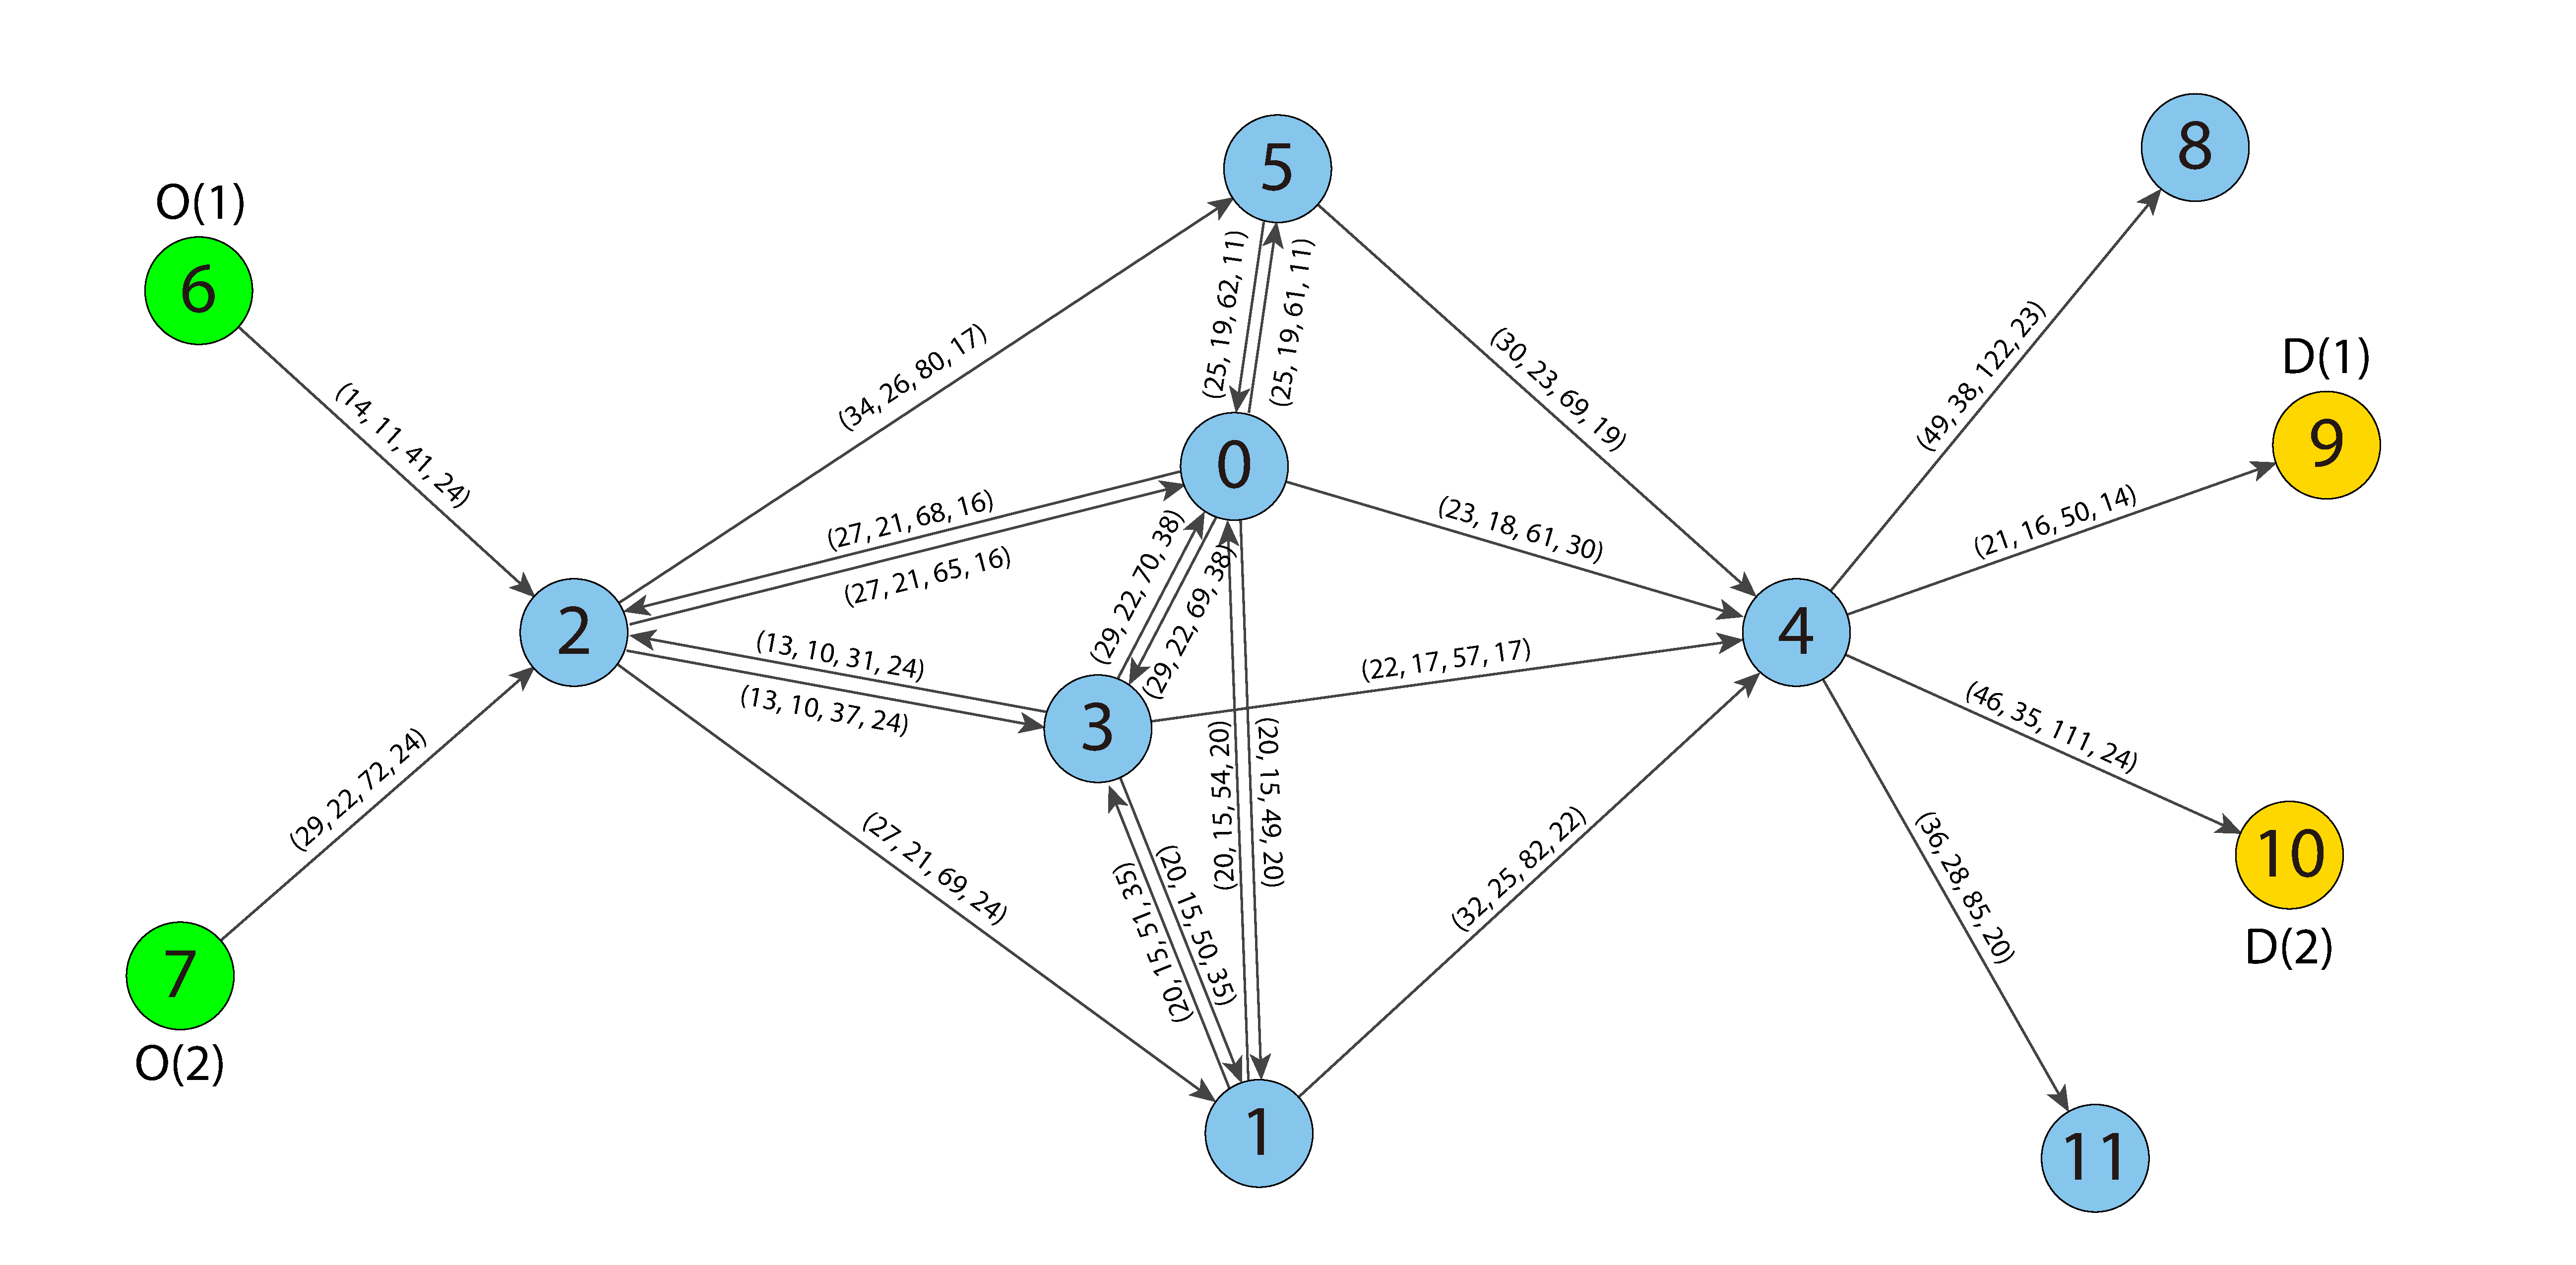
\includegraphics[width=\textwidth]{figures/Reinforcement/Example2.pdf}
    \caption{Example 2: a tuple on the edge represents $(c_{ij}^1, c_{ij}^2, f_{ij}, u_{ij})$}
    \label{fig:Example2}
\end{figure}
\clearpage

We define a global state $S_t \in \mathcal{S}$: $$S_t = (i_1, i_2, \boldsymbol{u}^t, \boldsymbol{y}^t) \in V \times V \times \mathbb{R}^{|E|} \times \{0,1\}^{|E|} = \mathcal{S},$$ with the following notations:
\begin{itemize}
    \item $i_k \in V$ for $k = 1,2$ is a node at which the agent $k$ is currently located
    \item $\boldsymbol{u}^t$ is a $|E|-$dimensional vector of $\{u_{(i,j)}^t\}_{(i,j)\in E}$, where $u_{(i,j)}^t$ is a remaining capacity of an edge $(i,j) \in E$ at time step $t$
    \item $\boldsymbol{y}^t$ is a $|E|-$dimensional vector of $\{y_{ij}^t\}_{(i,j)\in E}$, where $y_{ij}^t$ is a design variable on $(i,j)$ at time step $t$.
\end{itemize}

For $k = 1,2$, an action $A_t^{(k)}(s) \in \mathcal{A}^{(k)}$ available in state $S_t = (i_1, i_2, \boldsymbol{u}^t, \boldsymbol{y}^t)$ is to choose an edge $(i_k, j_k)$ where $$j_k \in \{j_k \in V \ | \ (i_k, j_k) \in E \text{ and } d^k \leq u^t_{i_k j_k}\} = \mathcal{A}^{(k)}(S_t).$$

%We note that it is hard to define how to calculate the remaining capacity when there exists an edge that has been visited by the same agent more than two times. To prevent this situation, we let agents follow a path only, meaning that it is not allowed to select an edge $(i_k,j_k)$ whose target node $j_k$ has already been visited by the agent $k$.

In order that the capacity constraints \eqref{eq:Capacity constraints} are not violated, we add the following setup. At each time step, if there exists an edge whose capacity constraint is violated by agents' actions, the agents who cause this situation bounce back to their original position. For example, at time step $t$, if two agents simultaneously choose the same edge $(i,j)$ whose current capacity $u_{ij}^t$ is less than the sum of their quantity $d^1 + d^2$, then both agents stay in the node $i$ at the next time step $t+1$.

We now discuss a reward function for \hyperref[fig:Example2]{Example 2}. Since we consider a deterministic environment, we have:
$$r(s,z) = r(s, z, s'),$$
where $s' = (i_1', i_2', \boldsymbol{u}', \boldsymbol{y}')= \tau(s,z)$. Then we define a reward function as follows:
\begin{align}
    r(s,z,s') = - \left(r_f + \sum_{k=1}^
    Kr_k\right),
\end{align}
where\footnote{Here $\{y_{ij}'\}_{(i,j)\in E}$ denote elements of $\boldsymbol{y}'$} \begin{align}
    r_f &= \sum_{(i,j)\in E}(y'_{ij}-y_{ij}) \cdot f_{ij}\\
    r_k &= \begin{cases}
    \beta &\text{if } i_k = i_k'\\
    c_{i_k i_k'}\cdot d^k &\text{if } i_k \neq i_k'
    \end{cases} \quad \text{for all } k \in \mathcal{K}
\end{align}
with a punishment factor $\beta \in \mathbb{R}_{>0}$.
\clearpage
\section{Value-based Methods}
In this section, we introduce


\subsection{Independent Q-learning}
Independent Q-learning (IQL) (\citeauthor{tan1993multi} \cite{tan1993multi}) is one of the pioneering approach to learning in the multi-agent settings. In IQL, each agent acts independently while the rest of agents are considered as part of the environment. In other words, each agent cannot observe other agents' action choice, while the reward function and the state-transition function depend on both a global state and actions of all agents. Thus, the environment becomes non-stationary from the perspective of each agent.

\subsection{Distributed Q-learning}
Distributed Q-learning (\citeauthor{lauer2000algorithm} \cite{lauer2000algorithm}) is an extension of IQL, where learning is distributed among agents. One can also say that the learning is decentralized. Let us split a policy $\Pi$ into $M$ agent-individual policies $\pi^{(m)}(s): \mathcal{S} \rightarrow \mathcal{A}^{(m)}$ with $\Pi(s) = (\pi^{(1)}(s), \dots, \pi^{(m)}(s), \dots,  \pi^{(M)}(s))$. Then a decentralized learning means that we learn each policy $\pi^{(m)}$ individually. \citeauthor{lauer2000algorithm} \cite{lauer2000algorithm} consider cooperative Markov games in their paper, and prove that their algorithm can find an optimal policy $\Pi_\ast$ in deterministic environments.

The main idea of distributed Q-learning is to properly compress the information of the central Q-table $Q(s,z)$ of size $|\mathcal{S}| \times |\mathcal{Z}|$ to the $M$ small, agent-individual tables $q^{(m)}(s,a^{(m)}$ of size $|\mathcal{S}| \times |\mathcal{A}^{(m)}|$.



The distributed Q-learning is comprised of two iteration rules. The first one is an algorithm that creates the small, agent-individual $q^{(m)}$-tables, describes as:
\begin{align}
    q_0^{(m)} &= 0\nonumber\\
    q_{t+1}^{(m)}(s,a^{(m)}) &=
    \begin{cases}
        q_t^{(m)}(s,a^{(m)}) &\mbox{if } s\neq S_t \text{ or }\\ & \quad a^{(m)}\neq A_t^{(m)}\\
    \max\{q_t^{(m)}(s,a^{(m)}), \\ \qquad r(S_t,Z_t) + \beta \cdot \underset{\tilde{a}^{(m)}\in\mathcal{A}^{(m)}}{\text{max}}q_t^{(m)}(S_{t+1}, \tilde{a}^{(m)})\} & \mbox{otherwise,}
    \end{cases}
\end{align}
where $A_t^{(m)}$ is agent $m$'s action choice at time step $t$, and $Z_t$ is the joint action of all agents at time step $t$.


The other one is an update rule for each agent-individual policy $\pi^{(m)}$.
\begin{align}
\pi_0^{(m)}(s) &\in \mathcal{A}^{(m)} \text{ arbitrarily }\nonumber\\
\pi_{t+1}^{(m)}(s) &= \begin{cases}
\pi_t^{(m)}(s) &\mbox{if }s\neq S_t \text{ or }\\
& \underset{a^{(m)}\in\mathcal{A}^{(m)}}{\text{max}}q_t^{(m)}(s,a^{(m)}) = \underset{a^{(m)}\in\mathcal{A}^{(m)}}{\text{max}}q_{t+1}^{(m)}(s,a^{(m)})\\
a_t^{(m)} &\mbox{otherwise}
\end{cases}
\end{align}




\section{Policy-based Methods}










%\part{Results}
\label{part:res}

\section{Validation of virtual reality setup}
\blindtext[3]      % INCLUDE Results
%\part{Discussion}
\label{part:disc}
\vspace*{3cm}
\section{Summary of findings}
\Blindtext[1]
\vfill   % INCLUDE Discussion
%\chapter{Conclusion}
\label{chap:con}
\Blindtext[2]
   % INCLUDE Conclusion
%\chapter{Perspectives}
\label{chap:persp}
The development of a virtual reality setup brings about exciting possibilities. Hopefully, we will soon see ants express innate behaviours such as searching, navigation, associative learning, etc. without moving in physical space. Coupled with the potential of exploring the neural basis of these behaviours is very promising indeed.
To enable this, I believe work should be targeted in two directions: \\ \\
\textbf{Implement new virtual reality software}. The current software (ViRMEn) has allowed us to probe the use of virtual reality with wood ants, however, it imposes certain limitations in the long term. It is written in Matlab, and customising it has remained a challenge throughout. Furthermore, one is limited to simple virtual environments created within ViRMEn. There are other potential software solutions openly available, e.g. MouseoVeR/FlyOver from Janelia Research Campus \autocite{Cohen2017MouseoVeRLaboratory}. This software is written in the open source programming language Python, and uses environments created in the open source 3D software, Blender. Not only will adopting this solution improve our ability to customise experiments to our needs, it will also improve the reproducibility by being based solely on open source software. \\ \\
\textbf{Develop reward system}. Associative learning experiments entails establishing an association between a cue and a reward (e.g. \cite{Fernandes2017a}), as does traditional navigation experiments with central place foragers (e.g. \cite{Buehlmann2018TheCharacteristics}). To allow such behaviour, the setup needs to allow distribution of reward. This could potentially be accomplished by introducing a syringe with a sucrose solution, however, this approach will first have to be developed and validated before beginning any learning experiments.  INCLUDE Perspectives


% -------------------------- 
% Back matter
% --------------------------
\chapter{References}
\vspace{1cm}
\printbibliography[heading=none]
%\chapter{Appendix}
\label{chap:appendix}

\section{Random graph generation: A complex network approach}
As we mentioned in section!!!!!!!!!!! \ref{S2V-DQL}, a collection of graph instances is needed for our method, S2V-DQN, to learn the evaluation function $\widehat{Q}$. In order to generate the graph instances, we use complex models which have been widely applied in modelling various real network systems such as World Wide Web (WWW), social networks, and ecological networks (\citeauthor{albert2002} \cite{albert2002}). The study of complex networks was initiated by \citeauthor{erdHos1960} \cite{erdHos1960}, who proposed a random graph model where, given $N$ nodes, $n$ arcs are selected from $N(N-1)/2$ allowable arcs with probability $p$. The random graph established by Erd{\H{o}}s and R{\'e}nyi \cite{erdHos1960} is referred to here as the ER model. This was then followed by two commonly used models: the Watts-Strogatz (WS) model (\citeauthor{watts1998} \cite{watts1998}) and the Barab\'asi-Albert (BA) model  (\citeauthor{barabasi1999emergence} \cite{barabasi1999emergence}). We will discuss these models in the following sections. The random graph theory is reveiwed in detail by \citeauthor{bollobas2001random} \cite{bollobas2001random} and \citeauthor{albert2002} \cite{albert2002}. Prior to formulating the complex network models, we first present fundamental measures and properties of complex networks.

\subsection{Network structure measures and properties}
We assume that a complex network is represented by a graph $G = (V, A)$, where $V$ is a set of nodes, $A$ is a set of arcs connecting two nodes in $V$, $|V| = N,$ and $|A| = M$. In the framework of random graph theory, the arcs are assumed to be  randomly distributed.

\subsubsection{Degree distribution}
Let $k_i$ denote the number of adjacent arcs of node $i$, which is called a \textit{degree} of node $i$. For the node degree $k$, we can then define a distribution function $P(k)$, which states the probability for node $i$ to be associated with $k$ arcs. The average degree of a network model is denoted by $\langle k \rangle$, which indicates the average number of neighbours of nodes in the network. \citeauthor{bollobas2001random} \cite{bollobas2001random} showed that the degree distribution of the ER model approaches a Poisson distribution. In other words, the number of nodes of degree $k$ in the network, denoted by $X_k$, has asymptotically Poisson distribution. \citeauthor{barabasi1999emergence} \cite{barabasi1999emergence}, however, discovered that many large networks in the real world such as WWW and citation patterns in science follow the \textit{scale-free} power law distribution, $P(k) \sim k^{-\gamma}$. We call such network \textit{scale-free} model.

\subsubsection{Average path length}\\
In order to quantify the structural features of complex networks \citeauthor{watts1998} \cite{watts1998} proposed two measures: \textit{average path length} and \textit{clustering coefficient}. The average path length, $\langle l \rangle$, calculates the average number of arcs in the shortest path over all pairs of nodes. This measure quantifies the global property of the network, in the sense that it estimates the separation between two nodes in the network model (\citeauthor{watts1998} \cite{watts1998}).

\subsubsection{Clustering coefficient}\\
The other structure measure introduced by \citeauthor{watts1998} \cite{watts1998} is clustering coefficient, denoted by $C_i$, which implies the local property of network model. Let us consider $k_i$ nearest neighbors of node $i$. Then there are $k_i(k_i-1)/2$ possible arcs between these $k_i$ nodes. For node $i$, the clustering coefficient then computes the fraction of these all possible arcs that actually exists in the model,
$$C_i = \frac{2E_i}{k_i(k_i-1)},$$
where $E_i$ is the number of arcs between the $k_i$ nearest neighbours of the node $i$. The average clustering coefficient of a network model $C$ is defined as
$$C = \frac{1}{N}\sum_{i=1}^{N}C_i,$$
which describes the ``cliquishness'' of given network model (\citeauthor{watts1998} \cite{watts1998}).

\subsubsection{Small-world}\\
The small-world concept states that any two nodes in large networks have short path lengths (\citeauthor{watts1998} \cite{watts1998}). \citeauthor{watts1998} \cite{watts1998} argue that this phenomenon can be found in real situations such as neural networks and power grids, and proposed the WS model that captures such small-world feature.

\subsection{Barab\'asi-Albert model}
Soon after the studies on the small-world model published by \citeauthor{watts1998} \cite{watts1998}, \citeauthor{barabasi1999emergence} \cite{barabasi1999emergence} proposed the scale-free model, which is referred to here as the BA model. The authors characterize the BA model by two key properties of real networks: \textit{growth} and \textit{preferential attachment}. The former indicates that the number of nodes in the model increases throughout the lifetime of the system by adding new nodes. The latter describes that a node with a larger number of connections has higher probability of being linked to the new nodes. \citeauthor{barabasi1999emergence} \cite{barabasi1999emergence} argue that the BA model displays the scale-free feature due to these two important properties, whereas the scale-free distribution is not observed from the two existing models - the ER model and the WS model.

The algorithm of the BA model from \citeauthor{barabasi1999emergence} \cite{barabasi1999emergence} can be formulated as follows:

\textit{Growth}\\
Let $m_0$ denote the cardinality of the initial set of nodes. At every time step $t$, one new node is added and connected to $m$ different nodes that already exist in the network. After t time steps, $mt$ arcs are added to the system with $N = t + m_0$ nodes.

\textit{Preferential attachment}\\
\citeauthor{barabasi1999emergence} \cite{barabasi1999emergence} define the probability $\Pi$ that newly added nodes choose the arc associated with node $i$ as the following:
$$\Pi(k_i) = \frac{k_i}{\sum_{j}k_j}$$
\citeauthor{barabasi1999mean} \cite{barabasi1999mean} showed that the degree distribution $P(k)$ of the BA model is asymptotically $P(k) \sim 2m^2k^{-3}$, indicating that it displays the scale-free feature.

\subsection{Supply chain networks}
Motivated by the development of complex network theory, there have been many studies analyzing the network structure of various real systems such as communication networks and ecological webs (\citeauthor{albert2002} \cite{albert2002}). The structure of supply chain network, in particular, has been investigated by \citeauthor{hearnshaw2013complex}  \cite{hearnshaw2013complex}. The authors suggested that efficient supply chains have a short average path length $\langle l \rangle$, a high clustering coefficient $C$, and a power law connectivity distribution. Based on this argument, it has been derived that the scale-free models better represent the properties of efficient supply chain than the WS model or the ER model, despite its limitations including low clustering coefficient. Their conceptual findings can be observed from a number of empirical studies exploring the topological structure of transportation networks (\citeauthor{tarapata2015modelling} \cite{tarapata2015modelling}; \citeauthor{haznagy2015complex} \cite{haznagy2015complex}; \citeauthor{de2019public} \cite{de2019public}).
% ********************************************************* 
% END OF THESIS
% *********************************************************
\end{document}